\documentclass[conference]{IEEEtran}
\usepackage[utf8]{inputenc}
\usepackage[T1]{fontenc}
\usepackage{amsmath}
\usepackage{amssymb}
\usepackage{graphicx}
\usepackage{url}

\begin{document}

\title{Classification bay\'esienne supervis\'ee de pixels : analyse des espaces colorim\'etriques RGB, HSV et Y$'$CbCr}


\author{
    \IEEEauthorblockN{1\textsuperscript{st} Santiago Florido Gomez}
    \IEEEauthorblockA{\textit{Ingénieur Degree Programme STIC} \\
    \textit{ENSTA Paris}\\
    Paris, France \\
    santiago.florido@ensta.fr}
    \and
    \IEEEauthorblockN{2\textsuperscript{nd} Javier Andres Tarazona Jimenez}
    \IEEEauthorblockA{\textit{Ingénieur Degree Programme STIC} \\
    \textit{ENSTA Paris}\\
    Paris, France \\
    javier-andres.tarazona@ensta.fr}
    \and
    \IEEEauthorblockN{3\textsuperscript{rd} José Daniel Chacón Gómez}
    \IEEEauthorblockA{\textit{Ingénieur Degree Programme STIC} \\
    \textit{ENSTA Paris}\\
    Paris, France \\
    jose-daniel.chacon@ensta.fr}
}

\maketitle

\begin{abstract}
Ce travail pr\'esente un cadre de classification bay\'esienne supervis\'ee appliqu\'e \`a la segmentation de pixels en imagerie couleur. L'article formalise les crit\`eres de d\'ecision Maximum A Posteriori (MAP) et Maximum Vraisemblance (ML), puis \'etudie le r\^ole du choix de l'espace d'observation dans la s\'eparabilit\'e statistique des classes. Trois repr\'esentations colorim\'etriques sont analys\'ees : RGB, HSV et Y$'$CbCr. Nous d\'ecrivons leurs transformations, leurs propri\'et\'es pertinentes pour l'inf\'erence probabiliste, et l'extraction op\'erationnelle de leurs composantes au moyen d'une impl\'ementation Python/OpenCV. Les visualisations et canaux export\'es (\texttt{R,G,B}, \texttt{H,S,V}, \texttt{Y',Cb,Cr}) fournissent une base reproductible pour la construction de mod\`eles bay\'esiens de classification de pixels et la comparaison de performances entre espaces colorim\'etriques.
\end{abstract}

\begin{IEEEkeywords}
Classification bay\'esienne, Maximum A Posteriori, Maximum Vraisemblance, segmentation de pixels, RGB, HSV, Y$'$CbCr, OpenCV.
\end{IEEEkeywords}
\section{Convolutional neural networks et CIFAR-10}
Dans le contexte de la classification d’images, les réseaux de neurones convolutionnels se sont consolidés comme l’une des architectures les plus adaptées à l’analyse des données visuelles, car ils permettent l’extraction automatique de caractéristiques spatiales hiérarchiques à partir des données d’entrée. Un réseau neuronal implémenté peut être modélisé comme une application composée
\begin{equation}
f_{\theta}:\mathbb{R}^{H\times W\times C}\rightarrow \mathbb{R}^{K},
\label{eq:cnn_mapping}
\end{equation}
où $H$ et $W$ sont la hauteur et la largeur de l’image, $C$ est le nombre de canaux, $K$ est le nombre de classes et $\theta$ désigne l’ensemble des paramètres entraînables.

Cette architecture remplace la connexion dense d’un réseau totalement connecté par une structure à champs réceptifs locaux, partage de poids et extraction hiérarchique de caractéristiques. Une CNN est organisée en plusieurs étapes, et chaque étape contient essentiellement une couche de filtres, une non-linéarité et une opération de réduction ou de \textit{pooling} sur des cartes de caractéristiques \cite{lecun_convolutional_networks}.

Soit $a^{(0)}=x$ l’entrée. Dans une couche convolutionnelle $l$, si l’entrée possède $C_{l-1}$ cartes et la sortie possède $C_l$ cartes, l’opération peut s’écrire
\begin{equation}
z^{(l)}_{i,j,m}
=
b^{(l)}_{m}
+
\sum_{c=1}^{C_{l-1}}
\sum_{u=0}^{k_h-1}
\sum_{v=0}^{k_w-1}
K^{(l)}_{u,v,c,m}\,
a^{(l-1)}_{i+u,\;j+v,\;c},
\label{eq:conv_layer}
\end{equation}
et, après la convolution, une non-linéarité ponctuelle est appliquée :
\begin{equation}
a^{(l)}_{i,j,m}
=
\phi\!\left(z^{(l)}_{i,j,m}\right).
\label{eq:nonlinearity}
\end{equation}

La dimension spatiale de la sortie d’une convolution avec pas (\textit{stride}) $s$ et remplissage (\textit{padding}) $p$ est donnée par
\begin{equation}
H_l=
\left\lfloor
\frac{H_{l-1}+2p_h-k_h}{s_h}
\right\rfloor+1,
\qquad
W_l=
\left\lfloor
\frac{W_{l-1}+2p_w-k_w}{s_w}
\right\rfloor+1.
\label{eq:conv_output_size}
\end{equation}
Cela permet de contrôler la résolution spatiale à mesure que le signal traverse le réseau.

Si un réseau possède plusieurs couches, le champ réceptif effectif d’un neurone dans les couches profondes croît avec la profondeur. Une manière utile de le modéliser est donnée par la récurrence
\begin{equation}
R_1=k_1,
\qquad
R_l=R_{l-1}+(k_l-1)\prod_{t=1}^{l-1}s_t,
\label{eq:receptive_field}
\end{equation}
où $R_l$ est la taille du champ réceptif effectif dans la couche $l$.

L’un des principaux avantages quantitatifs de la convolution est son efficacité paramétrique. Si une couche convolutionnelle possède $C_{\text{in}}$ canaux d’entrée, $C_{\text{out}}$ canaux de sortie et des filtres de taille $k_h\times k_w$, alors le nombre de paramètres est
\begin{equation}
N_{\text{params}}^{\text{conv}}
=
\left(k_hk_wC_{\text{in}}+1\right)C_{\text{out}}.
\label{eq:conv_params}
\end{equation}
En revanche, une couche dense reliant une entrée de taille $n_{\text{in}}$ à une sortie de taille $n_{\text{out}}$ possède
\begin{equation}
N_{\text{params}}^{\text{fc}}
=
\left(n_{\text{in}}+1\right)n_{\text{out}}.
\label{eq:fc_params}
\end{equation}

Cette différence constitue un élément significatif dans la classification automatique d’images, puisqu’une image d’entrée peut contenir des milliers de variables, tandis que la convolution exploite leurs caractéristiques structurelles en évitant une croissance explosive du nombre de poids.

Dans l’étape finale de classification, la représentation obtenue par les couches convolutionnelles est aplatie ou agrégée globalement afin de produire un vecteur $h\in\mathbb{R}^{d}$. Ensuite, une couche affine calcule
\begin{equation}
z=Wh+b,
\qquad
z\in\mathbb{R}^{K},
\label{eq:affine_classifier}
\end{equation}
et la probabilité estimée pour la classe $k$ est obtenue au moyen de la fonction \textit{softmax} :
\begin{equation}
\hat{y}_k=
\frac{e^{z_k}}{\sum_{j=1}^{K}e^{z_j}}.
\label{eq:softmax}
\end{equation}
\cite{lecun_convolutional_networks}

Il est proposé d’utiliser la base de données CIFAR-10, largement employée dans l’évaluation des algorithmes de classification d’images, qui contient $60\,000$ images RGB de $32\times 32$ pixels réparties en $10$ classes, avec $6\,000$ images par classe. La partition standard comprend $50\,000$ images pour l’entraînement et $10\,000$ pour le test ; de plus, l’ensemble de test contient exactement $1\,000$ images par classe et l’ensemble d’entraînement en contient $5\,000$ par classe. Les classes sont \textit{airplane}, \textit{automobile}, \textit{bird}, \textit{cat}, \textit{deer}, \textit{dog}, \textit{frog}, \textit{horse}, \textit{ship} et \textit{truck} \cite{cifar10_dataset}, ce qui représente un scénario adéquat pour l’analyse des éléments fondamentaux de l’apprentissage profond avec des exigences computationnelles modérées.

Comme une partie de l’objectif de recherche consiste également à étudier de manière contrôlée l’influence de la préparation des données, de la définition de l’architecture, de la sélection des hyperparamètres et de la définition de la dynamique d’apprentissage sur la performance idéale du modèle implémenté, ce cadre expérimental se révèle particulièrement pertinent.




\section{Structuration des données}
\subsection{training, validation, test}
La division de la base de données constitue un élément méthodologique propre à l’apprentissage supervisé, de manière à isoler l’information destinée à l’ajustement des paramètres, à la sélection du modèle et à l’évaluation du modèle entraîné. L’ensemble d’entraînement est utilisé pour l’estimation des paramètres du réseau, l’ensemble de validation a pour objectif de mesurer la généralisation du modèle sans intervenir directement dans les actualisations des paramètres, et, enfin, l’ensemble de test sert à obtenir une estimation indépendante et non biaisée de la performance du modèle sur des données qu’il n’a pas vues.

L’objectif de cette séparation est d’éviter la fuite d’information, qui peut se produire lorsque les données d’évaluation du modèle ont été utilisées dans l’estimation des paramètres et dans la définition de celui-ci, afin de pouvoir disposer de véritables mesures de la capacité de généralisation du modèle entraîné.

\subsection{ fonction standardize}
La fonction \texttt{standardize} peut être comprise comme une standardisation spatiale réalisée image par image et canal par canal. Pour un ensemble d’images représenté par un tenseur $x\in\mathbb{R}^{N\times H\times W\times C}$, la fonction calcule, pour chaque image $n$ et pour chaque canal $c$, la moyenne $\mu_{n,c}$ et l’écart-type $\sigma_{n,c}$ sur les dimensions spatiales $(H,W)$, puis transforme chaque pixel selon l’expression~\eqref{eq:standardize_transform} :

\begin{equation}
x'_{n,i,j,c}=\frac{x_{n,i,j,c}-\mu_{n,c}}{\sigma_{n,c}}.
\label{eq:standardize_transform}
\end{equation}

L’implication de cette implémentation est que chaque canal de chaque image est recentré autour de zéro et redimensionné de sorte que la dispersion soit aussi proche que possible d’une dispersion unitaire. Cet effet d’homogénéisation de l’entrée, en termes de son échelle numérique, facilite le processus d’optimisation et peut être utile pour accroître la stabilité de l’entraînement, car, en réduisant les différences globales d’intensité et de contraste entre les images, la standardisation diminue la variabilité non informative mais présente dans les données d’entrée, de manière à favoriser l’apprentissage par le réseau des motifs structurels les plus pertinents.
\section{Architecture du réseau}
Dans cette architecture, on définit un réseau de neurones convolutionnel séquentiel composé d’une étape d’extraction de caractéristiques locales au moyen de la convolution, suivie de réductions dimensionnelles par \textit{max pooling}. La couche d’entrée est définie pour un tenseur d’entrée $32\times 32\times 3$,
où $32$ est la hauteur, $32$ la largeur et $3$ le nombre de canaux de couleur $(R,G,B)$. Cette couche n’apprend pas de paramètres ; elle fixe uniquement la forme attendue des données d’entrée du modèle \cite{keras_input_object}.

Ensuite, une première couche convolutionnelle est définie pour la première extraction des caractéristiques. La couche apprend $8$ filtres distincts, ce qui implique qu’à sa sortie elle aura $8$ cartes de caractéristiques. Une dimension de noyau $(3,3)$ est définie, et l’argument \texttt{padding="same"} est incorporé dans la définition, ce qui permet de préserver la résolution spatiale de l’image, de sorte que la sortie conserve une hauteur et une largeur égales à celles de l’entrée. Par conséquent, la sortie de cette couche a la taille
\begin{equation}
32\times 32\times 8.
\end{equation}

Une couche de \textit{dropout} est ajoutée, laquelle remplit la fonction de mécanisme de régularisation durant l’entraînement en annulant aléatoirement une fraction des activations des entrées. Néanmoins, puisque la valeur du \textit{dropout} est fixée par défaut à zéro, la couche ne modifie ni l’information ni la dimension du tenseur. Sa sortie demeure
\begin{equation}
32\times 32\times 8.
\end{equation}

On ajoute une couche de \textit{max pooling} qui a un \textit{pool size} $(2,2)$, ce qui implique qu’elle réduit la résolution spatiale en prenant la valeur maximale dans chaque fenêtre locale $2\times 2$. De cette manière, la sortie de cette couche est
\begin{equation}
16\times 16\times 8.
\end{equation}

On ajoute ensuite une couche qui convertit le vecteur tridimensionnel en un vecteur unidimensionnel de dimension
\begin{equation}
16\cdot 16\cdot 8 = 2048,
\end{equation}

puis une transformation \textit{fully connected} est implémentée au moyen d’une couche dense vers un espace latent de $64$ neurones :
\begin{equation}
\mathbf{h}=\mathrm{ReLU}(W\mathbf{x}+\mathbf{b}).
\end{equation}

De sorte que la sortie de cette couche est de taille $64$, on ajoute une deuxième couche de \textit{dropout} dans laquelle le \textit{rate} est fixé à $0$, pour finalement inclure une couche dense supplémentaire vers un espace latent de dimension $10$. Dans cette occasion, l’activation \textit{softmax} transforme les scores en une distribution de probabilité :
\begin{equation}
\hat{y}_k=\frac{e^{z_k}}{\sum_{j=1}^{10} e^{z_j}},
\qquad
k=1,\dots,10.
\end{equation}

Par conséquent, chaque composante de la sortie appartient à l’intervalle $[0,1]$ et la somme de toutes est égale à $1$. La classe prédite est celle associée à l’indice ayant la probabilité la plus élevée :
\begin{equation}
\hat{c}=\arg\max_k \hat{y}_k.
\end{equation}

Enfin, il y a une dernière couche de \textit{dropout} avec un taux égal à $0$.

Les paramètres entraînables sont ceux que le modèle met à jour durant l’entraînement au moyen de la rétropropagation et de l’optimisation, lesquels, dans le cas de la structure proposée, sont incorporés dans les couches convolutionnelles et denses, puisque des couches telles que \texttt{Input}, \texttt{Dropout}, \texttt{MaxPooling2D} et \texttt{Flatten} n’incorporent pas de paramètres entraînables dans leur définition. Dans le cas de la couche \texttt{Conv2D},

\begin{equation}
N_{\text{params}}=(k_h\cdot k_w\cdot C_{\text{in}}+1)\cdot C_{\text{out}},
\end{equation}

où $k_h$ et $k_w$ sont les dimensions du filtre, $C_{\text{in}}$ le nombre de canaux d’entrée, et $C_{\text{out}}$ le nombre de filtres de sortie. Ici,

\begin{equation}
k_h=3,\qquad k_w=3,\qquad C_{\text{in}}=3,\qquad C_{\text{out}}=8.
\end{equation}

Alors,

\begin{equation}
N_{\text{params}}=(3\cdot 3\cdot 3+1)\cdot 8=(27+1)\cdot 8=224.
\end{equation}

C’est-à-dire que cette couche possède $224$ paramètres entraînables, y compris le biais \cite{keras_conv2d}.

Pour sa part, dans la couche dense avec biais,

\begin{equation}
N_{\text{params}}=(n_{\text{in}}+1)\cdot n_{\text{out}},
\end{equation}

où $n_{\text{in}}$ est le nombre d’entrées et $n_{\text{out}}$ le nombre de neurones de sortie. Dans le cas de la structure proposée, on a deux couches denses :

\begin{equation}
N_{\text{params}}=(2048+1)\cdot 64=2049\cdot 64=131136,
\end{equation}

et

\begin{equation}
N_{\text{params}}=(64+1)\cdot 10=650.
\end{equation}

Ainsi, le nombre total de paramètres entraînables est

\begin{equation}
224+131136+650=132010.
\end{equation}

\section{Apprentissage}

\subsection{D\'efinitions : epoch, step, batch}
Conform\'ement au cours, l'apprentissage supervis\'e du CNN de la Section~III consiste \`a ajuster un ensemble de poids entra\^inables
\begin{equation}
W=\{w_{ij}\},
\end{equation}
sur l'ensemble d'apprentissage $A=\{(X_i,V_i)\}_{i=1}^{N}$, de mani\`ere \`a minimiser la loss empirique
\begin{equation}
\begin{aligned}
L_A(W)
&=
\frac{1}{N}
\sum_{i=1}^{N}
L\!\left(\mathrm{ForwardProp}(W,X_i),V_i\right),\\
\widehat{W}
&=
\arg\min_{W} L_A(W).
\end{aligned}
\label{eq:section4_training_objective}
\end{equation}
Lorsque $A$ est partitionn\'e en lots $A_b\subset A$, $|A_b|=B$, la loss associ\'ee \`a un lot est d\'efinie par
\begin{equation}
L_b(W)
=
\frac{1}{|A_b|}
\sum_{(X_i,V_i)\in A_b}
L\!\left(\mathrm{ForwardProp}(W,X_i),V_i\right).
\label{eq:section4_batch_loss}
\end{equation}
Cette normalisation par $|A_b|$ est retenue dans toute la section, car elle permet de comparer des batch sizes diff\'erents sans modifier artificiellement l'\'echelle num\'erique de la loss ; elle correspond en outre \`a la convention de r\'eduction \texttt{sum\_over\_batch\_size} utilis\'ee dans l'impl\'ementation Keras.

Une it\'eration d'optimisation sur un lot s'\'ecrit alors, pour chaque connexion $(i,j)$,
\begin{equation}
w_{ij}^{(t)} = w_{ij}^{(t-1)} - \epsilon \, \frac{\partial L_b}{\partial w_{ij}},
\label{eq:section4_batch_update}
\end{equation}
o\`u $\epsilon>0$ d\'esigne le pas d'apprentissage. Dans ce cadre, un \textit{batch} est un sous-ensemble $A_b$ de cardinalit\'e $B$, un \textit{step} est une mise \`a jour de la forme~\eqref{eq:section4_batch_update}, et une \textit{epoch} correspond \`a un parcours complet de la base d'apprentissage. Si $N$ exemples sont trait\'es avec des lots de taille $B$, le nombre de steps par epoch vaut
\begin{equation}
S(B)=\left\lceil\frac{N}{B}\right\rceil.
\label{eq:section4_steps_per_epoch}
\end{equation}
Le cours distingue alors trois r\'egimes~: $B=1$ correspond au gradient stochastique, $B=N$ au gradient par lots complets, et $1<B<N$ \`a l'apprentissage par mini-batches, qui recherche un compromis entre bruit du gradient, co\^ut calculatoire et vitesse de convergence \cite{manzanera_classification_apprentissage,poly_chap4_classifml}.

\subsection{Influence de la taille du batch}
\paragraph{Protocole exp\'erimental.}
La pr\'esente section ne red\'efinit ni les donn\'ees ni l'architecture~: le d\'ecoupage des sous-ensembles et la fonction \texttt{standardize} sont ceux de la Section~II, et le CNN entra\^in\'e est celui de la Section~III. Seuls les param\`etres d'apprentissage sont modifi\'es pour l'\'etude des batch sizes et des optimiseurs.

\begin{table}[htbp]
\centering
\caption{Protocole exp\'erimental de la Section~4.}
\label{tab:section4_protocol}
\resizebox{\linewidth}{!}{%
\begin{tabular}{|l|l|}
\hline
R\'ef\'erences amont & Section~II pour les donn\'ees et la standardisation ; Section~III pour l'architecture \\
\hline
Sous-ensembles utilis\'es & $5000$ images d'entra\^inement, $1000$ images de validation ; l'ensemble de test n'intervient pas dans cette section \\
\hline
Graine de partition & $42$ \\
\hline
Graines d'initialisation & $42$, $314$ \\
\hline
Comparaison des batch sizes & $B \in \{8,16,32,64,128\}$, $8$ epochs fixes, SGD avec $\epsilon=10^{-2}$ \\
\hline
Comparaison des optimiseurs & $B=32$, $8$ epochs fixes, m\^emes poids initiaux pour une m\^eme graine \\
\hline
Hyperparam\`etres optimiseurs & SGD~: $\epsilon=10^{-2}$ ; SGD+Momentum~: $\epsilon=10^{-2}$, $\beta=0.9$ ; Adam~: $\epsilon=10^{-3}$, $\beta_1=0.9$, $\beta_2=0.999$, $\eta=10^{-7}$ \\
\hline
Conventions temporelles & temps/step~: moyenne des temps mur mesur\'es sur les lots d'entra\^inement ; temps/epoch~: temps mur d'une epoch incluant la validation \\
\hline
\end{tabular}%
}
\end{table}

La comparaison de la taille du batch est conduite \`a nombre d'epochs fix\'e, et non \`a nombre de mises \`a jour fix\'e. Ce point est essentiel pour l'interpr\'etation~: sur $8$ epochs, le nombre total d'updates vaut $8S(B)$, soit $5000$, $2504$, $1256$, $632$ et $320$ pour $B=8$, $16$, $32$, $64$ et $128$. Les diff\'erences observ\'ees entre batch sizes combinent donc deux effets~: la variation de bruit du gradient et la variation du nombre total de mises \`a jour.

Dans le tableau~\ref{tab:section4_batch_timing}, le symbole $m\pm\sigma$ d\'esigne la moyenne empirique $m$ et l'\'ecart-type empirique $\sigma$~; pour le temps par step, l'agr\'egation porte sur l'ensemble des steps mesur\'es au cours des deux graines et des huit epochs, tandis que pour le temps par epoch elle porte sur l'ensemble des epochs observ\'ees. Les courbes de la figure~\ref{fig:section4_batch_curves} sont les moyennes calcul\'ees sur les deux graines.

\begin{table}[htbp]
\centering
\caption{Influence de la taille du batch sur les co\^uts temporels moyens.}
\label{tab:section4_batch_timing}
\resizebox{\linewidth}{!}{%
\begin{tabular}{|c|c|c|c|}
\hline
Batch size $B$ & Steps/epoch $S(B)$ & Temps moyen par step (s) & Temps moyen par epoch (s) \\
\hline
8 & 625 & 0.0052 $\pm$ 0.0107 & 3.882 $\pm$ 0.460 \\
16 & 313 & 0.0079 $\pm$ 0.0160 & 2.959 $\pm$ 0.391 \\
32 & 157 & 0.0117 $\pm$ 0.0234 & 2.234 $\pm$ 0.410 \\
64 & 79 & 0.0182 $\pm$ 0.0287 & 1.745 $\pm$ 0.371 \\
128 & 40 & 0.0297 $\pm$ 0.0383 & 1.457 $\pm$ 0.340 \\
\hline
\end{tabular}%
}
\end{table}

\begin{figure}[htbp]
\centering
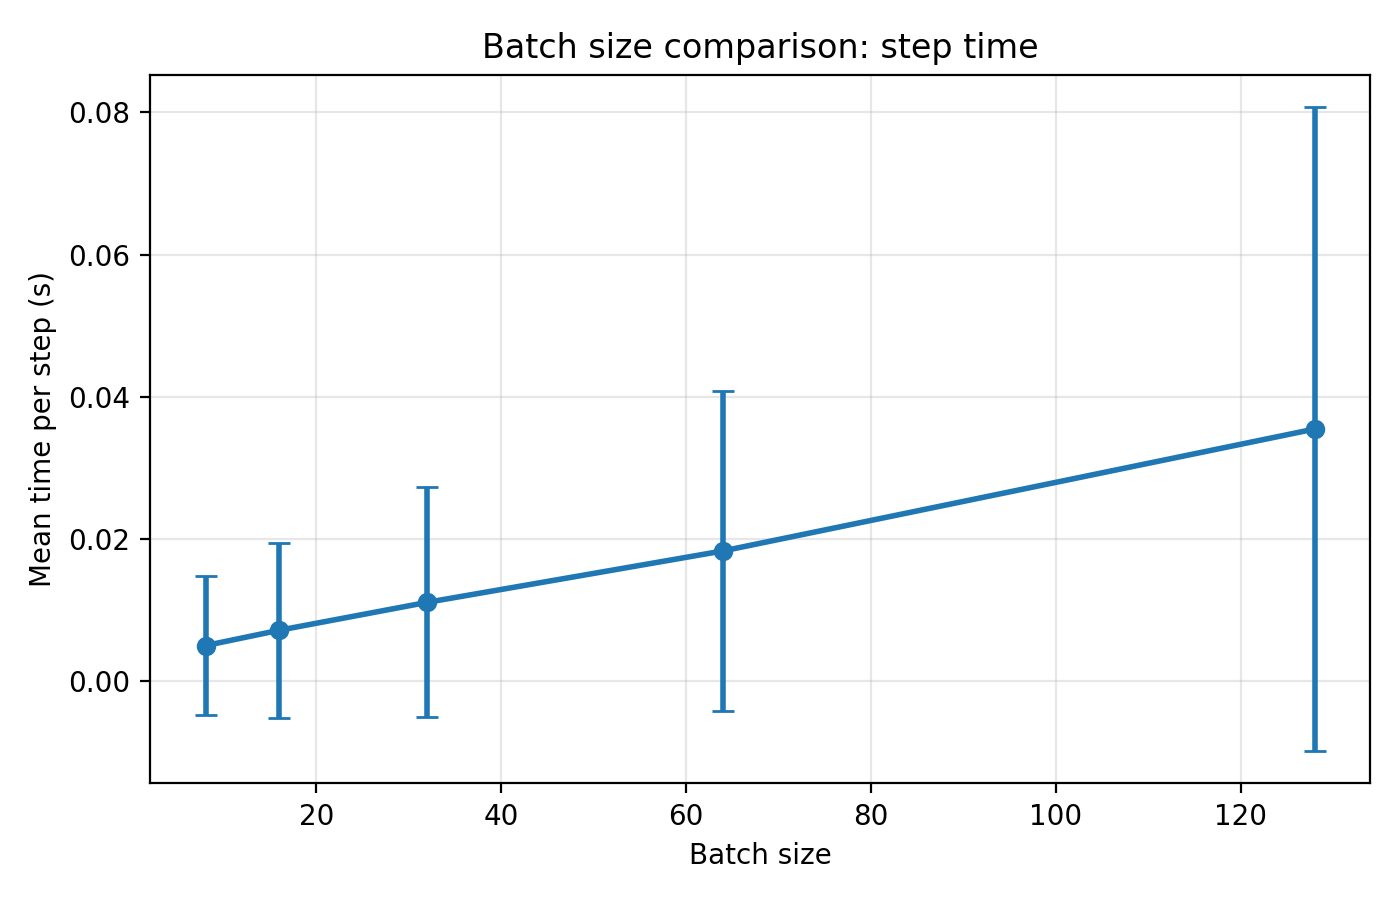
\includegraphics[width=\linewidth]{imgs/section4_batch_step_time.png}
\caption{Temps moyen par step en fonction de la taille du batch.}
\label{fig:section4_batch_step_time}
\end{figure}

\begin{figure}[htbp]
\centering
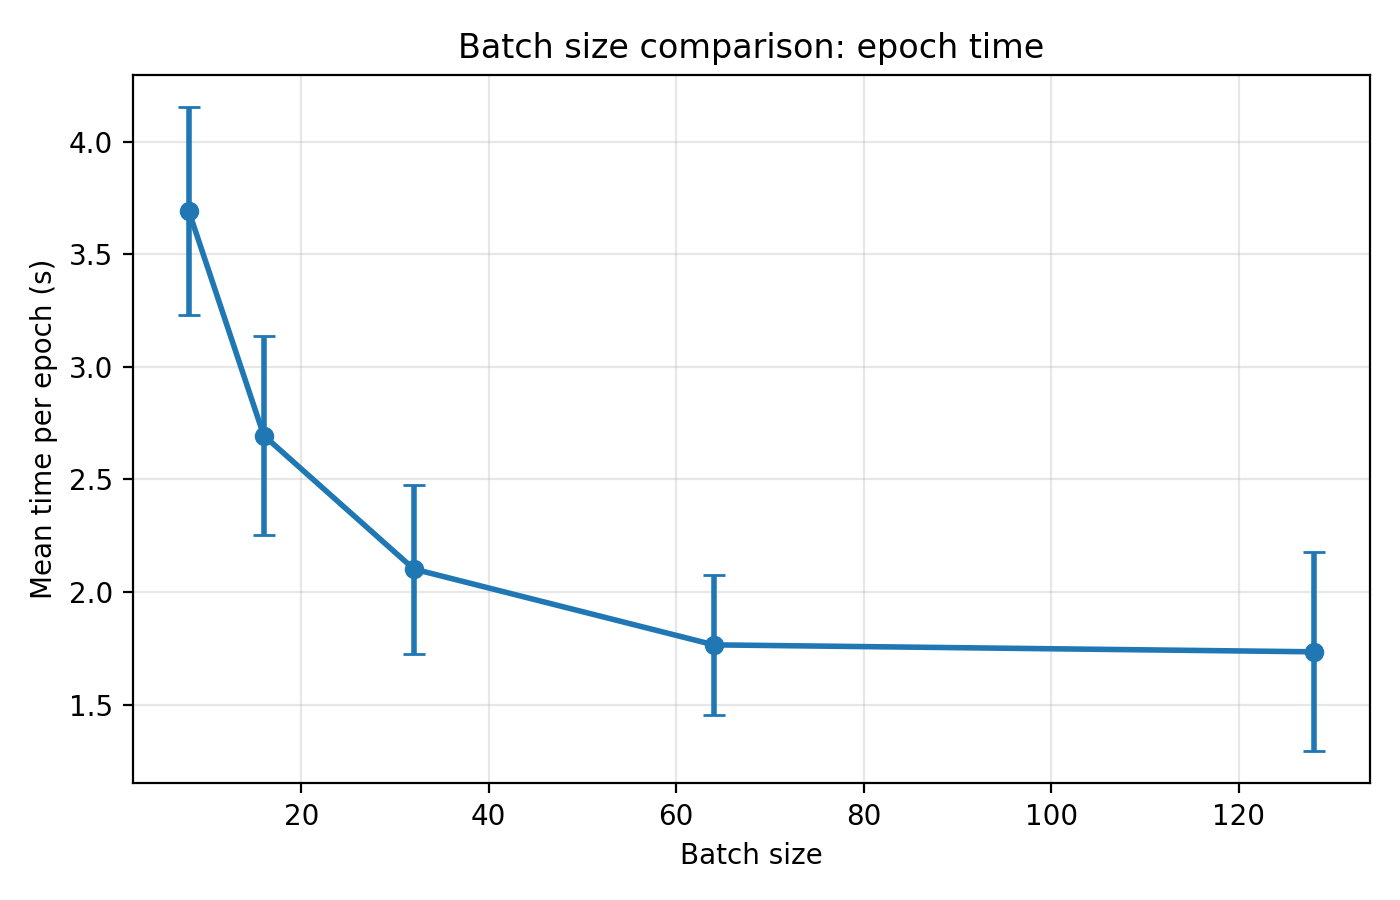
\includegraphics[width=\linewidth]{imgs/section4_batch_epoch_time.png}
\caption{Temps moyen par epoch en fonction de la taille du batch.}
\label{fig:section4_batch_epoch_time}
\end{figure}

Les figures~\ref{fig:section4_batch_step_time} et~\ref{fig:section4_batch_epoch_time} confirment la relation attendue par~\eqref{eq:section4_steps_per_epoch}. Le temps moyen par step cro\^it avec $B$, de $0.0052\,\mathrm{s}$ \`a $0.0297\,\mathrm{s}$, car chaque mise \`a jour traite davantage d'exemples. En sens inverse, le temps moyen par epoch d\'ecro\^it de $3.882\,\mathrm{s}$ \`a $1.457\,\mathrm{s}$, puisque le nombre de steps diminue fortement. Cette d\'ecroissance reste sous-lin\'eaire, ce qui est coh\'erent avec le cours~: l'augmentation de la taille du lot r\'eduit le nombre d'updates mais n'annule pas le surco\^ut de calcul de chaque update \cite{manzanera_classification_apprentissage,poly_chap4_classifml}.

\begin{figure}[htbp]
\centering
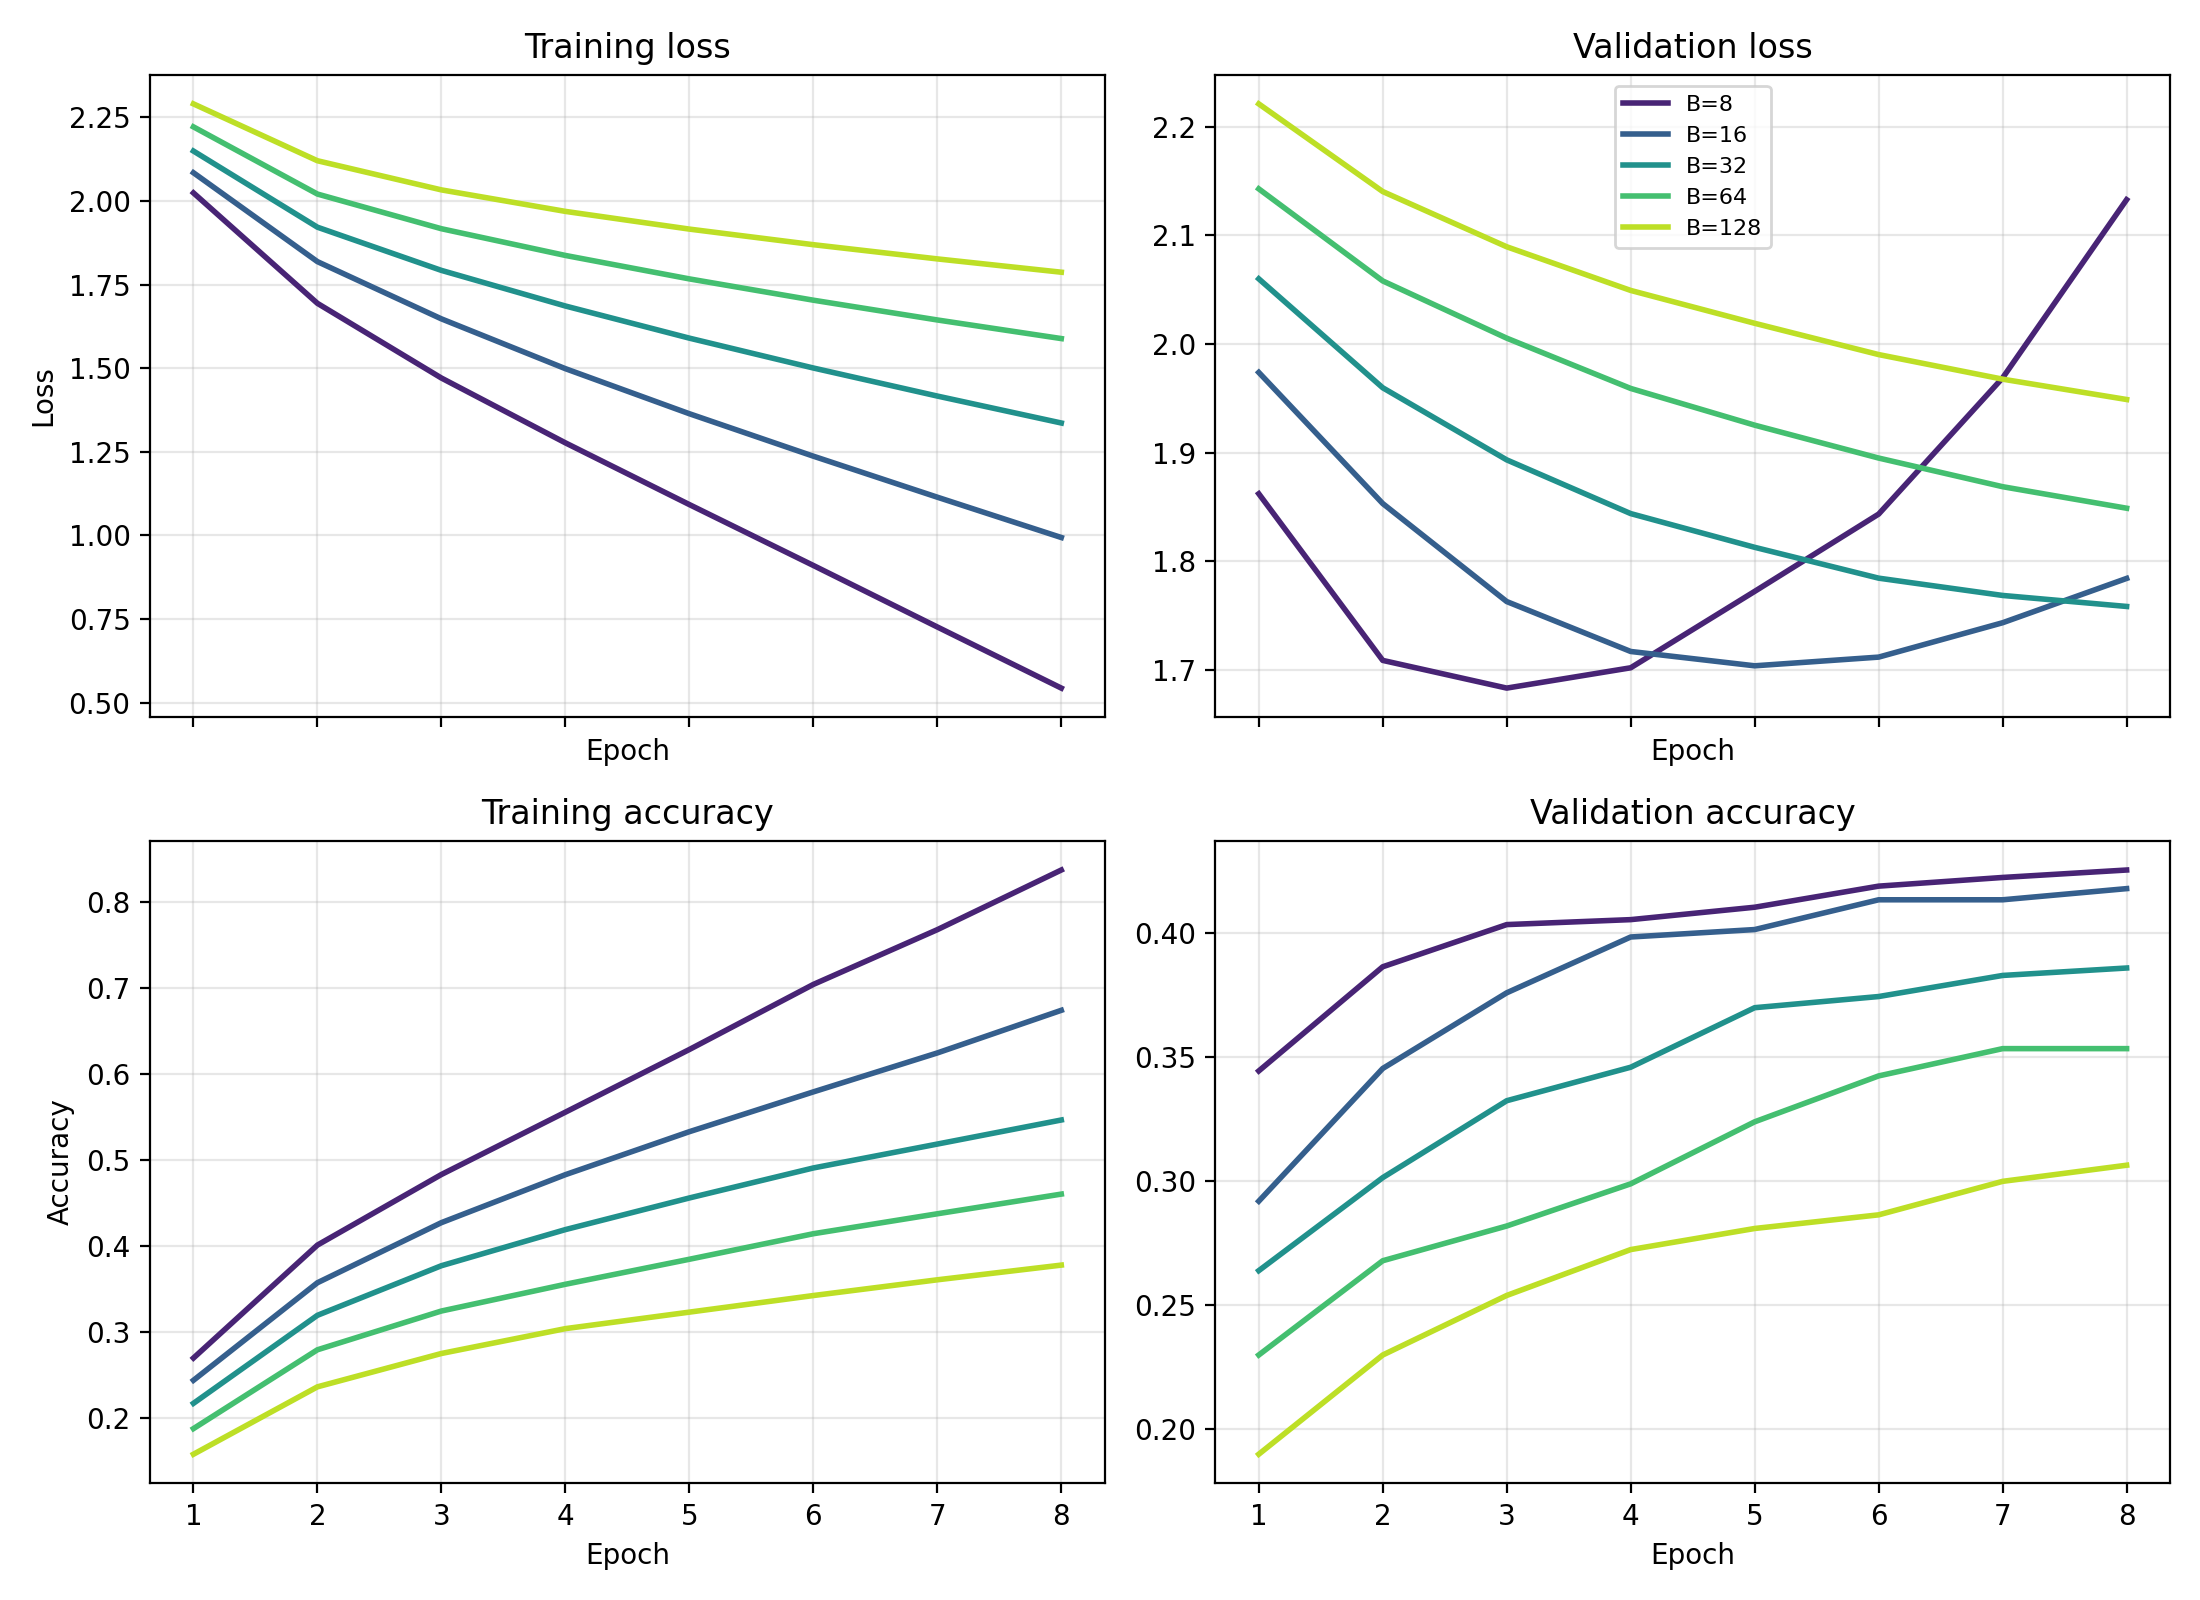
\includegraphics[width=\linewidth]{imgs/section4_batch_curves.png}
\caption{Courbes moyennes d'entra\^inement et de validation pour diff\'erentes tailles de batch.}
\label{fig:section4_batch_curves}
\end{figure}

L'interpr\'etation des courbes doit rester li\'ee au budget fix\'e en epochs. Dans ce cadre, les plus petits batches atteignent les meilleures accuracies de validation finales~: $42.55\%$ pour $B=8$ et $41.80\%$ pour $B=16$, contre $38.60\%$, $35.35\%$ et $30.65\%$ pour $B=32$, $64$ et $128$. Une partie de cet avantage provient du fait que les petits batches r\'ealisent un nombre nettement plus grand de mises \`a jour sur le m\^eme budget de $8$ epochs. En revanche, $B=8$ produit aussi la dynamique de validation la plus bruit\'ee~: la val. loss atteint un minimum moyen de $1.6833$ \`a l'epoch $3$, puis remonte jusqu'\`a $2.1329$ \`a l'epoch $8$. Sous le protocole consid\'er\'e, $B=16$ appara\^it ainsi comme la valeur la plus \'equilibr\'ee parmi celles test\'ees, en conservant une accuracy finale proche de $B=8$ avec des courbes de validation moins irr\'eguli\`eres et un temps par epoch plus faible.

\subsection{Comparaison des m\'ethodes d'optimisation}
Le SGD de base correspond directement \`a l'actualisation scalaire~\eqref{eq:section4_batch_update}, appliqu\'ee \`a chaque connexion $(i,j)$. Le cours pr\'esente ensuite le SGD avec Momentum sous la forme d'une accumulation des gradients successifs~; pour chaque poids $w_{ij}$,
\begin{equation}
G_t = \beta G_{t-1} + (1-\beta)\frac{\partial L_b}{\partial w_{ij}},
\qquad
w_{ij}^{(t)} = w_{ij}^{(t-1)} - \epsilon G_t.
\label{eq:section4_momentum}
\end{equation}
Le terme $G_t$ lisse ainsi les variations de direction du gradient d'un batch au suivant \cite{manzanera_classification_apprentissage,poly_chap4_classifml}.

Pour Adam, la pr\'esente section reprend explicitement l'\'ecriture simplifi\'ee du cours, sans correction de biais~:
\begin{equation}
G_t = \beta_1 G_{t-1} + (1-\beta_1)\frac{\partial L_b}{\partial w_{ij}},
\end{equation}
\begin{equation}
K_t = \beta_2 K_{t-1} + (1-\beta_2)\left(\frac{\partial L_b}{\partial w_{ij}}\right)^2,
\end{equation}
\begin{equation}
w_{ij}^{(t)} = w_{ij}^{(t-1)} - \epsilon \, \frac{G_t}{\sqrt{K_t}+\eta}.
\label{eq:section4_adam}
\end{equation}
Dans cette expression, $\epsilon$ d\'esigne le pas d'apprentissage, tandis que $\eta>0$ est le petit terme introduit au d\'enominateur pour \`eviter une division par z\'ero. Cette m\'ethode adapte donc, pour chaque poids, l'amplitude de la mise \`a jour tout en lissant les fluctuations temporelles du gradient.

La comparaison des optimiseurs est men\'ee \`a batch size fix\'e $B=32$ et \`a nombre d'epochs fix\'e ($8$). Le tableau~\ref{tab:section4_optimizer_summary} regroupe les statistiques agr\'eg\'ees sur les deux graines~; pour le temps par epoch, la notation $m\pm\sigma$ correspond \`a la moyenne et \`a l'\'ecart-type empiriques sur l'ensemble des epochs mesur\'ees, tandis que l'accuracy finale de validation et le minimum de val. loss sont moyenn\'es sur les deux graines.

\begin{table}[htbp]
\centering
\caption{Comparaison des optimiseurs \`a batch size fix\'e $B=32$. Le symbole $\pm$ d\'esigne l'\'ecart-type empirique du temps par epoch.}
\label{tab:section4_optimizer_summary}
\resizebox{\linewidth}{!}{%
\begin{tabular}{|c|c|c|c|}
\hline
Optimiseur & Temps moyen par epoch (s) & Accuracy finale de validation (\%) & Minimum de la val. loss \\
\hline
SGD & 2.133 $\pm$ 0.334 & 38.60 & 1.7584 \\
SGD+Momentum & 2.240 $\pm$ 0.493 & 40.20 & 1.7079 \\
Adam & 2.417 $\pm$ 0.755 & 43.45 & 1.6083 \\
\hline
\end{tabular}%
}
\end{table}

\begin{figure}[htbp]
\centering
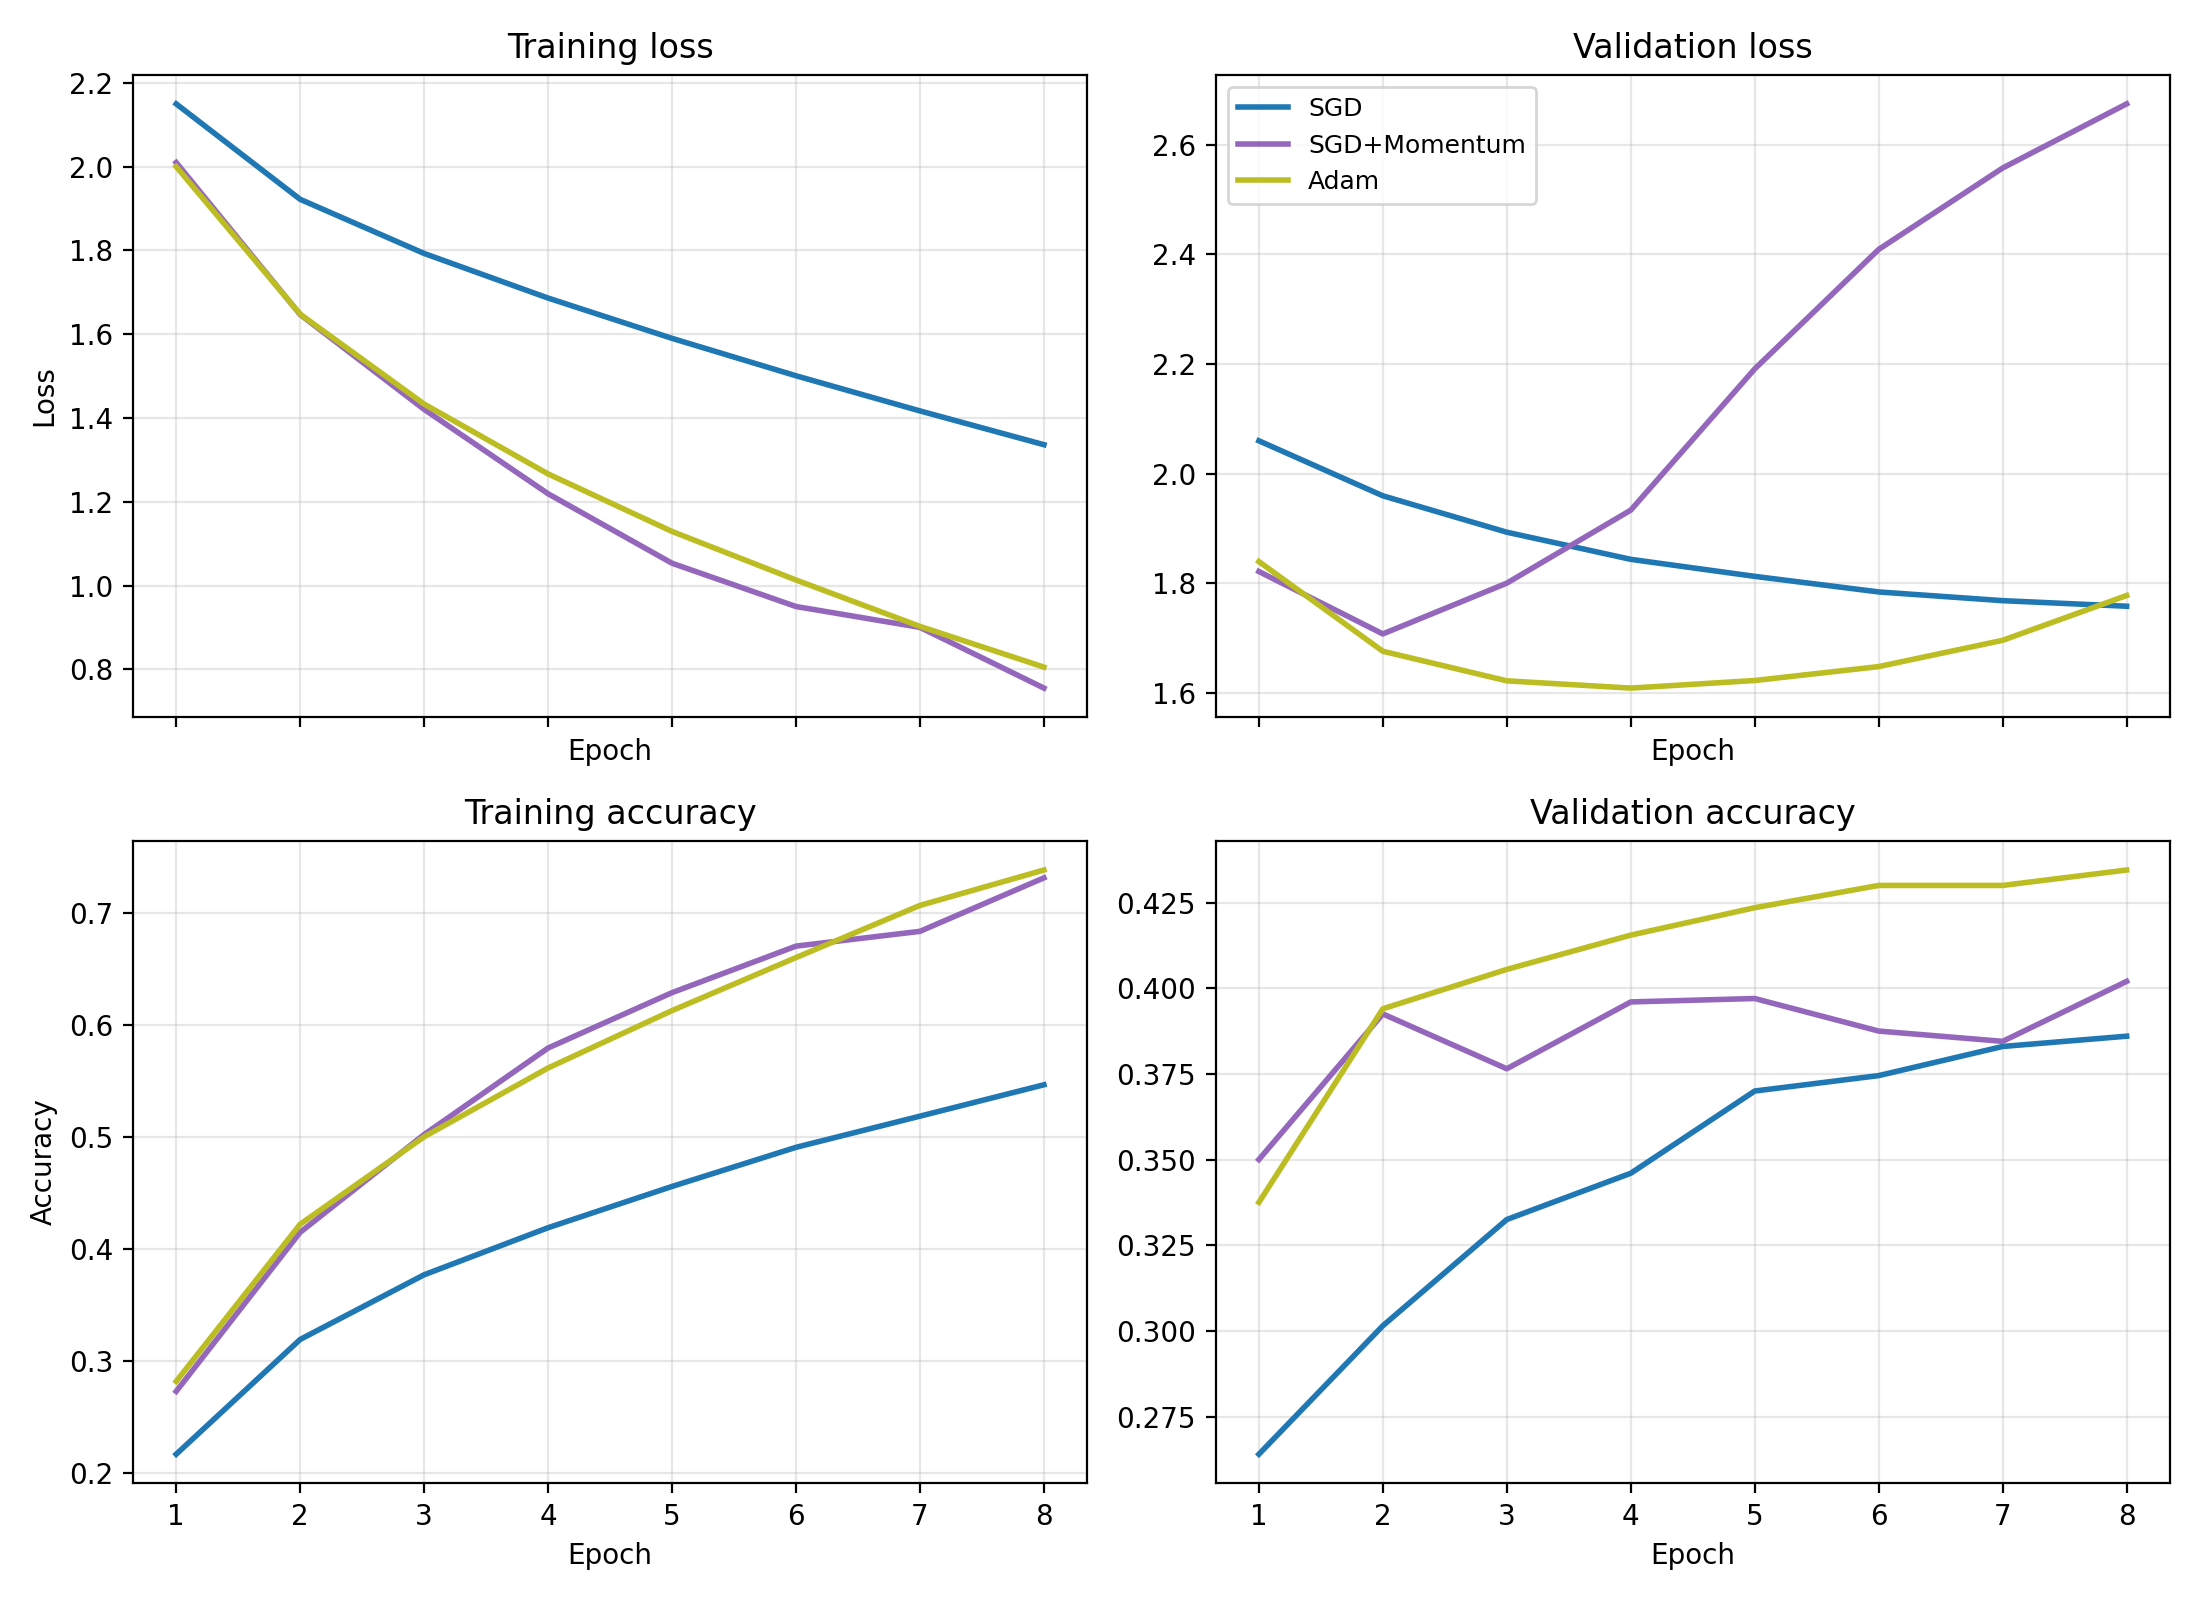
\includegraphics[width=\linewidth]{imgs/section4_optimizer_curves.png}
\caption{Courbes moyennes d'entra\^inement et de validation pour SGD, SGD+Momentum et Adam.}
\label{fig:section4_optimizer_curves}
\end{figure}

Sous ce protocole, le SGD fournit la d\'ecroissance de validation la plus r\'eguli\`ere~: la val. loss baisse presque monotoniquement jusqu'\`a $1.7584$, pour une accuracy finale de $38.60\%$. Le Momentum acc\'el\`ere la descente initiale, avec un minimum moyen de val. loss \`a $1.7079$ d\`es l'epoch $2$, mais la remont\'ee ult\'erieure jusqu'\`a $2.6743$ \`a l'epoch $8$ indique une d\'egradation plus marqu\'ee en fin d'entra\^inement. Cette observation est coh\'erente avec l'interpr\'etation du cours~: le terme $G_t$ stabilise les directions du gradient, mais peut aussi prolonger des mises \`a jour devenues trop agressives lorsque $\epsilon$ reste fix\'e.

Parmi les trois optimiseurs test\'es, Adam obtient les meilleures m\'etriques de validation dans le cadre pr\'esent~: accuracy finale moyenne de $43.45\%$ et minimum moyen de val. loss de $1.6083$. Le surco\^ut temporel reste mod\'er\'e ($2.417\,\mathrm{s}$ par epoch contre $2.133\,\mathrm{s}$ pour SGD), ce qui sugg\`ere que l'adaptation locale des mises \`a jour compense efficacement cette surcharge sur le budget calculatoire consid\'er\'e.

\subsection{Synth\`ese}
Sous le protocole \`a nombre d'epochs fix\'e retenu ici, la taille du batch agit simultan\'ement sur le bruit du gradient et sur le nombre total de mises \`a jour. Les petits batches favorisent donc la performance de validation, mais au prix de courbes plus bruit\'ees et d'un temps par epoch plus \'elev\'e ; parmi les valeurs test\'ees, $B=16$ fournit le compromis le plus favorable entre co\^ut temporel et qualit\'e de validation, tandis que $B=8$ donne l'accuracy finale la plus \'elev\'ee.

\paragraph{Limites exp\'erimentales.}
La port\'ee de ces conclusions reste limit\'ee au protocole \'etudi\'e~: sous-ensemble r\'eduit de CIFAR-10, CNN de taille modeste, apprentissage sur CPU et deux graines d'initialisation seulement. Dans ce cadre, Adam pr\'esente les meilleures m\'etriques de validation parmi les optimiseurs compar\'es, avec un surco\^ut temporel mod\'er\'e ; cette observation ne pr\'etend toutefois pas valoir ind\'ependamment de l'architecture, du budget d'updates ou du choix des hyperparam\`etres.

\section{Hyperparam\`etres}

\subsection{D\'efinition et distinction avec les param\`etres entra\^inables}
Contrairement aux poids du r\'eseau, d\'etaill\'es \`a la Section~III, les hyperparam\`etres ne sont pas appris par r\'etropropagation. Ils sont fix\'es avant ou autour de l'apprentissage et d\'eterminent l'architecture, la fonction objective, le sch\'ema d'optimisation, le protocole d'entra\^inement et la r\'egularisation \cite{poly_chap4_classifml,manzanera_classification_apprentissage}. Les poids $W=\{w_{ij}\}$ et les biais des couches convolutionnelles et denses sont, au contraire, ajust\'es pendant l'optimisation selon les \`equations de la Section~4.

Les quantit\'es de journalisation et de sauvegarde, telles que \texttt{verbose}, \texttt{filepath} ou les options de \texttt{ModelCheckpoint}, sont donc exclues de l'inventaire. Les tailles de sous-ensembles, les graines et le pr\'etraitement \texttt{standardize} influencent l'exp\'erience, mais ils sont trait\'es ici comme des conditions exp\'erimentales externes et non comme des hyperparam\`etres du mod\`ele au sens strict.

\subsection{Inventaire analytique des hyperparam\`etres}
L'inventaire est \`etabli directement \`a partir des appels du notebook et de la pipeline reproductible, en relevant explicitement des expressions telles que \texttt{Conv2D(filters=8, kernel\_size=(3,3), padding="same")}, \texttt{units} (Dense cach\'ee), \texttt{compile(loss="categorical\_crossentropy", optimizer=...)} et \texttt{fit(..., batch\_size=..., epochs=..., shuffle=True)}. Pour gagner en pr\'ecision, les hyperparam\`etres sont distingu\'es entre hyperparam\`etres structurels impos\'es par la t\^ache, hyperparam\`etres ajustables de conception, hyperparam\`etres d'entra\^inement et hyperparam\`etres de r\'egularisation.

\begin{table*}[t]
\centering
\caption{Inventaire d\'etaill\'e des hyperparam\`etres structurels, de conception et de r\'egularisation.}
\label{tab:section5_structure_inventory}
\scriptsize
\begin{tabular}{|p{2.6cm}|p{3.5cm}|p{3.1cm}|p{6.9cm}|}
\hline
Nom dans le code & Nature pr\'ecise & Valeur retenue & Influence attendue \\
\hline
\texttt{shape} & structurel impos\'e par la t\^ache & $32\times 32\times 3$ & fixe la forme des donn\'ees d'entr\'ee et contraint la premi\`ere couche du r\'eseau \\
\hline
\texttt{units} (sortie) & structurel impos\'e par la t\^ache & $10$ sorties & impose la dimension de sortie du classifieur, donc le nombre de classes trait\'ees \\
\hline
nombre de couches \texttt{Conv2D} & ajustable de conception & $1$ couche convolutionnelle & fixe la profondeur de l'extraction locale et contribue \`a la croissance du champ r\'ecepteur effectif \\
\hline
\texttt{filters} & ajustable de conception & $8$ & modifie la largeur de la repr\'esentation convolutionnelle et le nombre de poids appris \\
\hline
\texttt{kernel\_size} & ajustable de conception & $(3,3)$ & contr\^ole le voisinage local explor\'e et participe directement au champ r\'ecepteur \\
\hline
\texttt{padding} & ajustable de conception & \texttt{same} & pr\'eserve la r\'esolution spatiale et conditionne la taille des tenseurs transmis aux couches suivantes \\
\hline
\texttt{pool\_size} & ajustable de conception & $(2,2)$ & r\'eduit la r\'esolution spatiale, le co\^ut calculatoire et agrandit le champ r\'ecepteur effectif des couches profondes \\
\hline
\texttt{Flatten} & ajustable de conception & \texttt{Flatten} & fixe la transition convolution/dense et donc la taille d'entr\'ee de la t\^ete de classification \\
\hline
\texttt{units} (Dense cach\'ee) & ajustable de conception & $64$ neurones & contr\^ole la largeur de la t\^ete dense et la capacit\'e expressive de la partie pleinement connect\'ee \\
\hline
\texttt{activation} (cach\'ee) & ajustable de conception & ReLU & introduit la non-lin\'earit\'e et limite en pratique l'att\'enuation du gradient dans les premi\`eres couches \\
\hline
\texttt{activation} (sortie) & ajustable de conception & softmax & rend la sortie compatible avec une interpr\'etation probabiliste et avec l'entropie crois\'ee \\
\hline
\texttt{rate} & r\'egularisation & $0.0$ & si le taux \`etait strictement positif, il r\'eduirait la co-adaptation des neurones ; ici son effet empirique est nul \\
\hline
\texttt{l2} & r\'egularisation & $\lambda_{L^2}=0.00$ & si le coefficient \`etait positif, il p\'enaliserait les poids trop grands ; ici son effet empirique est nul \\
\hline
\end{tabular}
\end{table*}

\begin{table*}[t]
\centering
\caption{Inventaire d\'etaill\'e des hyperparam\`etres d'entra\^inement.}
\label{tab:section5_training_inventory}
\scriptsize
\begin{tabular}{|p{2.2cm}|p{2.7cm}|p{2.5cm}|p{3.7cm}|p{5.5cm}|}
\hline
Nom dans le code & Nature pr\'ecise & Valeur initiale & Valeurs explor\'ees / retenues & Influence attendue \\
\hline
\texttt{loss} & entra\^inement & \shortstack[l]{\texttt{categorical\_}\\\texttt{crossentropy}} & valeur conserv\'ee dans tout le protocole & d\'efinit la quantit\'e dont le gradient pilote l'apprentissage ; ici elle est adapt\'ee \`a une sortie softmax et \`a des labels one-hot \\
\hline
\texttt{optimizer} & entra\^inement & SGD & SGD, SGD+Momentum, Adam & modifie la dynamique de convergence, le lissage des gradients et la sensibilit\'e au pas d'apprentissage \\
\hline
\texttt{learning\_rate} & entra\^inement & $0.01$ & $0.01$ pour SGD/SGD+Momentum ; $0.001$ pour Adam & multiplie directement le gradient dans les mises \`a jour ; trop grand, il destabilise la descente ; trop faible, il ralentit la convergence \\
\hline
\texttt{momentum} & entra\^inement & $0.0$ & $0.0$ puis $0.9$ & ajoute une inertie directionnelle qui lisse les fluctuations du gradient entre deux mini-batches \\
\hline
\texttt{beta\_1} & entra\^inement & -- & $0.9$ pour Adam & contr\^ole le lissage du premier moment dans Adam \\
\hline
\texttt{beta\_2} & entra\^inement & -- & $0.999$ pour Adam & contr\^ole le lissage du second moment dans Adam \\
\hline
\texttt{epsilon} d'Adam & entra\^inement & -- & $10^{-7}$ pour Adam & stabilise num\'eriquement le d\'enominateur de l'update d'Adam ; il correspond au terme not\'e $\eta$ dans le rapport \\
\hline
\texttt{batch\_size} & entra\^inement & $32$ & $8$ ; puis $\{8,16,32,64,128\}$ ; $32$ retenu pour l'\'etude des optimiseurs & agit sur le bruit du gradient, le nombre d'updates par epoch et le compromis entre stabilit\'e et co\^ut calculatoire \\
\hline
\texttt{epochs} & entra\^inement & $20$ & $10$ ; puis $8$ retenu pour les comparaisons contr\^ol\'ees & fixe le budget d'apprentissage en passages sur la base et conditionne le niveau de convergence atteint \\
\hline
\texttt{shuffle} & entra\^inement & valeur par d\'efaut dans le notebook & \texttt{True} dans la pipeline reproductible & limite les effets d'ordre entre epochs et stabilise l'estimation du gradient stochastique \\
\hline
\end{tabular}
\end{table*}

Les tailles de sous-ensembles, les graines de partition ou d'initialisation et le pr\'etraitement \texttt{standardize} ne figurent pas dans les Tables~\ref{tab:section5_structure_inventory} et~\ref{tab:section5_training_inventory}. Ces quantit\'es modifient bien les conditions d'observation et la variance des r\'esultats, mais elles ne constituent pas des hyperparam\`etres sintonisables du mod\`ele lui-m\^eme.

\subsection{Influence des principaux hyperparam\`etres sur l'apprentissage}
\paragraph{Hyperparam\`etres d'optimisation.}
Les hyperparam\`etres d'optimisation ont d\'ej\`a fait l'objet d'une \`etude empirique en Section~4 ; ils sont seulement replac\'es ici dans une typologie g\'en\'erale. Dans \eqref{eq:section4_batch_update}, le pas d'apprentissage $\epsilon$ multiplie directement le gradient. Un $\epsilon$ trop grand peut donc provoquer des oscillations ou faire franchir une zone de minimum ; un $\epsilon$ trop faible ralentit au contraire la convergence et augmente le co\^ut calculatoire. Le choix de l'optimiseur modifie ensuite la mani\`ere dont cette actualisation est liss\'ee ou repond\'er\'ee : le Momentum introduit une inertie directionnelle, tandis qu'Adam adapte localement l'amplitude des mises \`a jour. La taille du batch, le nombre d'epochs et \texttt{shuffle} gouvernent enfin le bruit du gradient, le budget d'actualisations et les effets d'ordre entre mini-batches.

\paragraph{Hyperparam\`etres d'architecture.}
Les hyperparam\`etres d'architecture d\'ej\`a d\'ecrits en Section~III deviennent ici des quantit\'es de conception ajustables. Augmenter le nombre de filtres ou la dimension de la couche dense accro\^it la capacit\'e de repr\'esentation du r\'eseau, mais aussi le nombre de poids \`a estimer. Le noyau convolutionnel et le \textit{pooling} contr\^olent en outre le champ r\'ecepteur effectif des neurones profonds : via \eqref{eq:receptive_field}, ils d\'eterminent la portion du contexte spatial initial que les derni\`eres couches peuvent analyser pour prendre une d\'ecision. Un champ r\'ecepteur trop petit limite l'acc\`es au contexte global, alors qu'un champ plus large favorise l'int\'egration spatiale au prix d'un co\^ut calculatoire et param\'etrique plus \`elev\'e.

\paragraph{Hyperparam\`etres de r\'egularisation.}
Le dropout et la p\'enalisation $L^2$ doivent \^etre analys\'es m\^eme lorsque leurs valeurs sont nulles dans le code. Un taux de dropout strictement positif force le r\'eseau \`a ne pas d\'ependre d'un petit nombre de neurones particuliers, ce qui limite la co-adaptation et r\'eduit le risque de sur-apprentissage. La p\'enalisation $L^2$, ou \textit{weight decay}, d\'ecourage les poids trop grands et tend \`a lisser le mod\`ele. Ces deux quantit\'es sont donc bien des hyperparam\`etres de r\'egularisation au sens du mod\`ele, mais elles ne participent pas aux r\'esultats observ\'es dans le protocole courant puisque leurs valeurs sont nulles.

\subsection{Synth\`ese}
La Section~V rel\`eve les hyperparam\`etres du projet un par un, avec leur nom exact dans le code, leur nature et leur influence attendue. Les hyperparam\`etres structurels impos\'es par la t\^ache doivent \^etre distingu\'es des hyperparam\`etres ajustables de conception, d'entra\^inement et de r\'egularisation. Les tailles de sous-ensembles, les graines et le pr\'etraitement conditionnent l'exp\'erience, mais ils rel\`event de conditions exp\'erimentales externes plut\^ot que d'hyperparam\`etres du mod\`ele lui-m\^eme.

\section{Approfondissement du mod\`ele}

\subsection{Limites du mod\`ele de base et objectif du raffinement}
Le mod\`ele de base d\'ecrit en Section~III repose sur une seule couche convolutionnelle suivie d'un \textit{flattening} et d'une t\^ete dense. Cette structure reste valide pour une premi\`ere \'etude, mais elle pr\'esente trois limites nettes pour la classification sur CIFAR-10. D'abord, l'extraction de caract\'eristiques demeure peu hi\'erarchique, puisqu'une seule convolution est appliqu\'ee avant la d\'ecision. Ensuite, l'essentiel des param\`etres entra\^inables est concentr\'e dans la partie dense : sur $132010$ param\`etres, $131786$ appartiennent \`a la t\^ete dense, contre seulement $224$ pour la couche convolutionnelle. Enfin, aucune r\'egularisation effective n'intervient dans cette baseline, puisque les taux de \textit{dropout} et les coefficients $L^2$ sont nuls.

Les architectures convolutionnelles sont pourtant motiv\'ees, dans le cadre du cours, par l'id\'ee d'une extraction locale et invariante par translation au moyen d'un banc de filtres, combin\'ee \`a des m\'ecanismes de r\'eduction spatiale par \textit{pooling} ou \textit{stride} \cite{manzanera_classification_apprentissage,poly_chap4_classifml,lecun_convolutional_networks}. L'approfondissement du r\'eseau doit donc permettre \`a la fois d\'augmenter le champ r\'ecepteur effectif, de construire des repr\'esentations plus abstraites et de r\'e\'equilibrer la r\'epartition des param\`etres entre la partie convolutionnelle et la partie d\'ecisionnelle. L'objectif de cette section consiste ainsi \`a concevoir une architecture plus profonde, \`a en v\'erifier la coh\'erence dimensionnelle, puis \`a mesurer rigoureusement si le gain de performance justifie la complexit\'e suppl\'ementaire.

\subsection{Conception d'une architecture convolutionnelle plus profonde}
Le raffinement a \'et\'e men\'e \`a partir de trois variantes plus profondes que la baseline. La premi\`ere, not\'ee $M1$, ajoute une deuxi\`eme \'etape convolutionnelle et porte la profondeur \`a quatre convolutions. La deuxi\`eme, not\'ee $M2$, ajoute une troisi\`eme \'etape convolutionnelle, ce qui porte la profondeur \`a six convolutions et r\'eduit la r\'esolution finale \`a $4\times 4$. La troisi\`eme, not\'ee $M3$, reprend exactement le squelette de $M2$ mais y ajoute une r\'egularisation explicite : \textit{dropout} de $0.25$ apr\`es chaque \textit{pooling}, \textit{dropout} de $0.5$ avant la couche dense cach\'ee et p\'enalisation $L^2$ de coefficient $10^{-4}$.

Cette progression respecte l'interpr\'etation du cours : les couches convolutionnelles successives apprennent des \textit{features} de complexit\'e croissante, tandis que les couches de \textit{pooling} r\'eduisent la r\'esolution spatiale et augmentent la port\'ee contextuelle des neurones profonds \cite{poly_chap4_classifml}. Le choix de noyaux $3\times 3$ conserv\'es \`a toutes les couches maintient un calcul local simple, tandis que la multiplication des \'etapes convolutionnelles permet d\'agrandir progressivement le champ r\'ecepteur sans introduire de filtres tr\`es larges. Le tableau~\ref{tab:section6_architectures} r\'esume les variantes compar\'ees.

\begin{table*}[htbp]
\centering
\caption{Architectures compar\'ees pour l'approfondissement du mod\`ele.}
\label{tab:section6_architectures}
\small
\begin{tabular}{|c|l|l|c|}
\hline
Mod\`ele & Backbone convolutionnel & R\'egularisation & Param\`etres \\
\hline
$M0$ & $8$/pool & aucune & $132010$ \\
$M1$ & $16$-$16$/pool $\rightarrow$ $32$-$32$/pool & aucune & $148442$ \\
$M2$ & $16$-$16$/pool $\rightarrow$ $32$-$32$/pool $\rightarrow$ $64$-$64$/pool & aucune & $138330$ \\
$M3$ & $16$-$16$/pool $\rightarrow$ $32$-$32$/pool $\rightarrow$ $64$-$64$/pool & dropout $0.25/0.25/0.25$, dropout dense $0.5$, $L^2=10^{-4}$ & $138330$ \\
\hline
\end{tabular}
\end{table*}

Deux observations ressortent imm\'ediatement. D'une part, $M1$ poss\`ede davantage de param\`etres que $M3$, bien qu'il soit moins profond ; cela provient du fait que deux seuls \textit{poolings} laissent une carte finale de taille $8\times 8\times 32$, soit un \textit{flattening} de dimension $2048$, alors que $M3$ descend \`a $4\times 4\times 64$, soit une dimension $1024$ avant la partie dense. D'autre part, $M2$ et $M3$ ont exactement le m\^eme nombre de param\`etres, puisque \textit{dropout} et p\'enalisation $L^2$ n'ajoutent pas de poids entra\^inables.

\subsection{Coh\'erence dimensionnelle des tenseurs}
La coh\'erence entre les tenseurs d'entr\'ee et de sortie a \'et\'e contr\^ol\'ee explicitement pour toutes les architectures. Si une couche re\c coit un tenseur $H_l \times W_l \times C_l$, alors une convolution $3\times 3$ avec \texttt{padding="same"} et pas $1$ produit un tenseur $H_l \times W_l \times F_l$, o\`u $F_l$ d\'esigne le nombre de filtres. Un \textit{max pooling} $2\times 2$ de pas $2$ produit ensuite un tenseur
\begin{equation}
\frac{H_l}{2} \times \frac{W_l}{2} \times C_l,
\end{equation}
ce qui impose que les dimensions spatiales restent compatibles avec les r\'eductions successives.

Pour le mod\`ele finalement retenu, la cha\^ine dimensionnelle s'\'ecrit :
\begin{equation}
\resizebox{0.98\columnwidth}{!}{$
\begin{aligned}
32\times 32\times 3 &\rightarrow 32\times 32\times 16 \rightarrow 32\times 32\times 16 \rightarrow 16\times 16\times 16, \\
16\times 16\times 16 &\rightarrow 16\times 16\times 32 \rightarrow 16\times 16\times 32 \rightarrow 8\times 8\times 32, \\
8\times 8\times 32 &\rightarrow 8\times 8\times 64 \rightarrow 8\times 8\times 64 \rightarrow 4\times 4\times 64, \\
4\times 4\times 64 &\rightarrow 1024 \rightarrow 64 \rightarrow 10.
\end{aligned}$}
\end{equation}
Le tableau~\ref{tab:section6_dimensions} reprend cette progression couche par couche. La transition vers la partie dense demeure assur\'ee par un \textit{flattening}, conform\'ement au sch\'ema d\'ecrit dans le polycopi\'e pour les t\^aches de classification \`a sortie de taille fixe \cite{poly_chap4_classifml}.

\begin{table}[htbp]
\centering
\caption{Coh\'erence dimensionnelle du mod\`ele retenu $M3$.}
\label{tab:section6_dimensions}
\small
\begin{tabular}{|l|c|c|}
\hline
Couche & Sortie & Param\`etres \\
\hline
Input & $32\times 32\times 3$ & $0$ \\
Conv2D $(16)$ & $32\times 32\times 16$ & $448$ \\
Conv2D $(16)$ & $32\times 32\times 16$ & $2320$ \\
MaxPool2D & $16\times 16\times 16$ & $0$ \\
Conv2D $(32)$ & $16\times 16\times 32$ & $4640$ \\
Conv2D $(32)$ & $16\times 16\times 32$ & $9248$ \\
MaxPool2D & $8\times 8\times 32$ & $0$ \\
Conv2D $(64)$ & $8\times 8\times 64$ & $18496$ \\
Conv2D $(64)$ & $8\times 8\times 64$ & $36928$ \\
MaxPool2D & $4\times 4\times 64$ & $0$ \\
Flatten & $1024$ & $0$ \\
Dense & $64$ & $65600$ \\
Dense & $10$ & $650$ \\
\hline
\end{tabular}
\end{table}

\subsection{Protocole d'entra\^inement et comparaison contr\^ol\'ee}
La comparaison a conserv\'e exactement le protocole de donn\'ees de la Section~IV : m\^eme partition r\'eduite de CIFAR-10 ($5000$ images d'entra\^inement, $1000$ de validation, $1000$ de test), m\^eme standardisation image par image et m\^eme nombre de classes. Afin d'isoler autant que possible l'effet de l'architecture, l'optimiseur a \'et\'e fix\'e \`a Adam avec $(\epsilon,\beta_1,\beta_2,\eta)=(10^{-3},0.9,0.999,10^{-7})$, le \textit{batch size} \`a $32$ et le m\'elange des mini-batches \`a \texttt{True}.

La campagne a \'et\'e men\'ee en deux \'etapes. Un \textit{screening} initial a compar\'e les quatre architectures sur la graine $42$ pendant $10$ epochs. Les deux meilleures architectures raffin\'ees ont ensuite \'et\'e soumises \`a une phase de confirmation, avec les graines $42$ et $314$ et un budget de $12$ epochs. La r\`egle de s\'election a \'et\'e fix\'ee \textit{a priori} : accuracy finale de validation moyenne maximale, puis minimum moyen de \textit{val. loss}, puis temps moyen par epoch.

Le tableau~\ref{tab:section6_performance} rassemble les r\'esultats. Lors du \textit{screening}, $M3$ obtient la meilleure accuracy finale de validation ($48.10\%$), devant $M1$ ($46.20\%$), $M2$ ($43.60\%$) et la baseline $M0$ ($39.50\%$). L'int\'er\^et de la r\'egularisation appara\^it d\'ej\`a clairement : $M3$ surpasse $M2$ de $4.5$ points d\'accuracy finale, alors que les deux mod\`eles partagent exactement le m\^eme backbone convolutionnel.

La phase de confirmation confirme cette hi\'erarchie. $M3$ atteint une accuracy finale de validation moyenne de $50.80\% \pm 1.60$, avec un minimum moyen de \textit{val. loss} de $1.4073 \pm 0.0663$. $M1$ progresse lui aussi par rapport \`a la baseline, avec $48.55\% \pm 1.55$, mais reste en retrait. Le gain de $M3$ par rapport \`a $M0$ est de $8.5$ points d\'accuracy finale de validation, au prix d'un temps moyen par epoch qui passe de $1.256\,\mathrm{s}$ \`a $3.708\,\mathrm{s}$.

\begin{table*}[htbp]
\centering
\caption{Comparaison des architectures pendant le \textit{screening} et la confirmation. Pour la confirmation, le symbole $\pm$ d\'esigne l'\'ecart-type empirique sur les deux graines.}
\label{tab:section6_performance}
\small
\begin{tabular}{|c|c|c|c|c|c|c|}
\hline
Etape & Mod\`ele & Nb. conv & Param\`etres & Accuracy finale val. (\%) & Min. val. loss & Temps/epoch (s) \\
\hline
Screening & $M0$ & $1$ & $132010$ & $39.50$ & $1.6113$ & $1.346$ \\
Screening & $M1$ & $4$ & $148442$ & $46.20$ & $1.6386$ & $2.824$ \\
Screening & $M2$ & $6$ & $138330$ & $43.60$ & $1.6178$ & $3.463$ \\
Screening & $M3$ & $6$ & $138330$ & $48.10$ & $1.5431$ & $3.833$ \\
\hline
Confirmation & $M0$ & $1$ & $132010$ & $42.30 \pm 1.10$ & $1.6167 \pm 0.0055$ & $1.256 \pm 0.611$ \\
Confirmation & $M1$ & $4$ & $148442$ & $48.55 \pm 1.55$ & $1.5804 \pm 0.0582$ & $2.478 \pm 0.702$ \\
Confirmation & $M3$ & $6$ & $138330$ & $50.80 \pm 1.60$ & $1.4073 \pm 0.0663$ & $3.708 \pm 1.453$ \\
\hline
\end{tabular}
\end{table*}

\subsection{Mod\`ele final retenu : architecture, hyperparam\`etres, courbes et matrices de confusion}
Au vu de la phase de confirmation, $M3$ a \'et\'e retenu comme mod\`ele final. La figure~\ref{fig:section6_architecture} en donne une repr\'esentation graphique, et le tableau~\ref{tab:section6_hyperparameters} en synth\'etise les hyperparam\`etres effectifs. La profondeur convolutionnelle y est port\'ee \`a six couches, r\'eparties sur trois \'etapes de largeur croissante $(16,32,64)$, avec trois r\'eductions spatiales successives et une t\^ete dense de dimension $64$.

\begin{figure}[htbp]
\centering
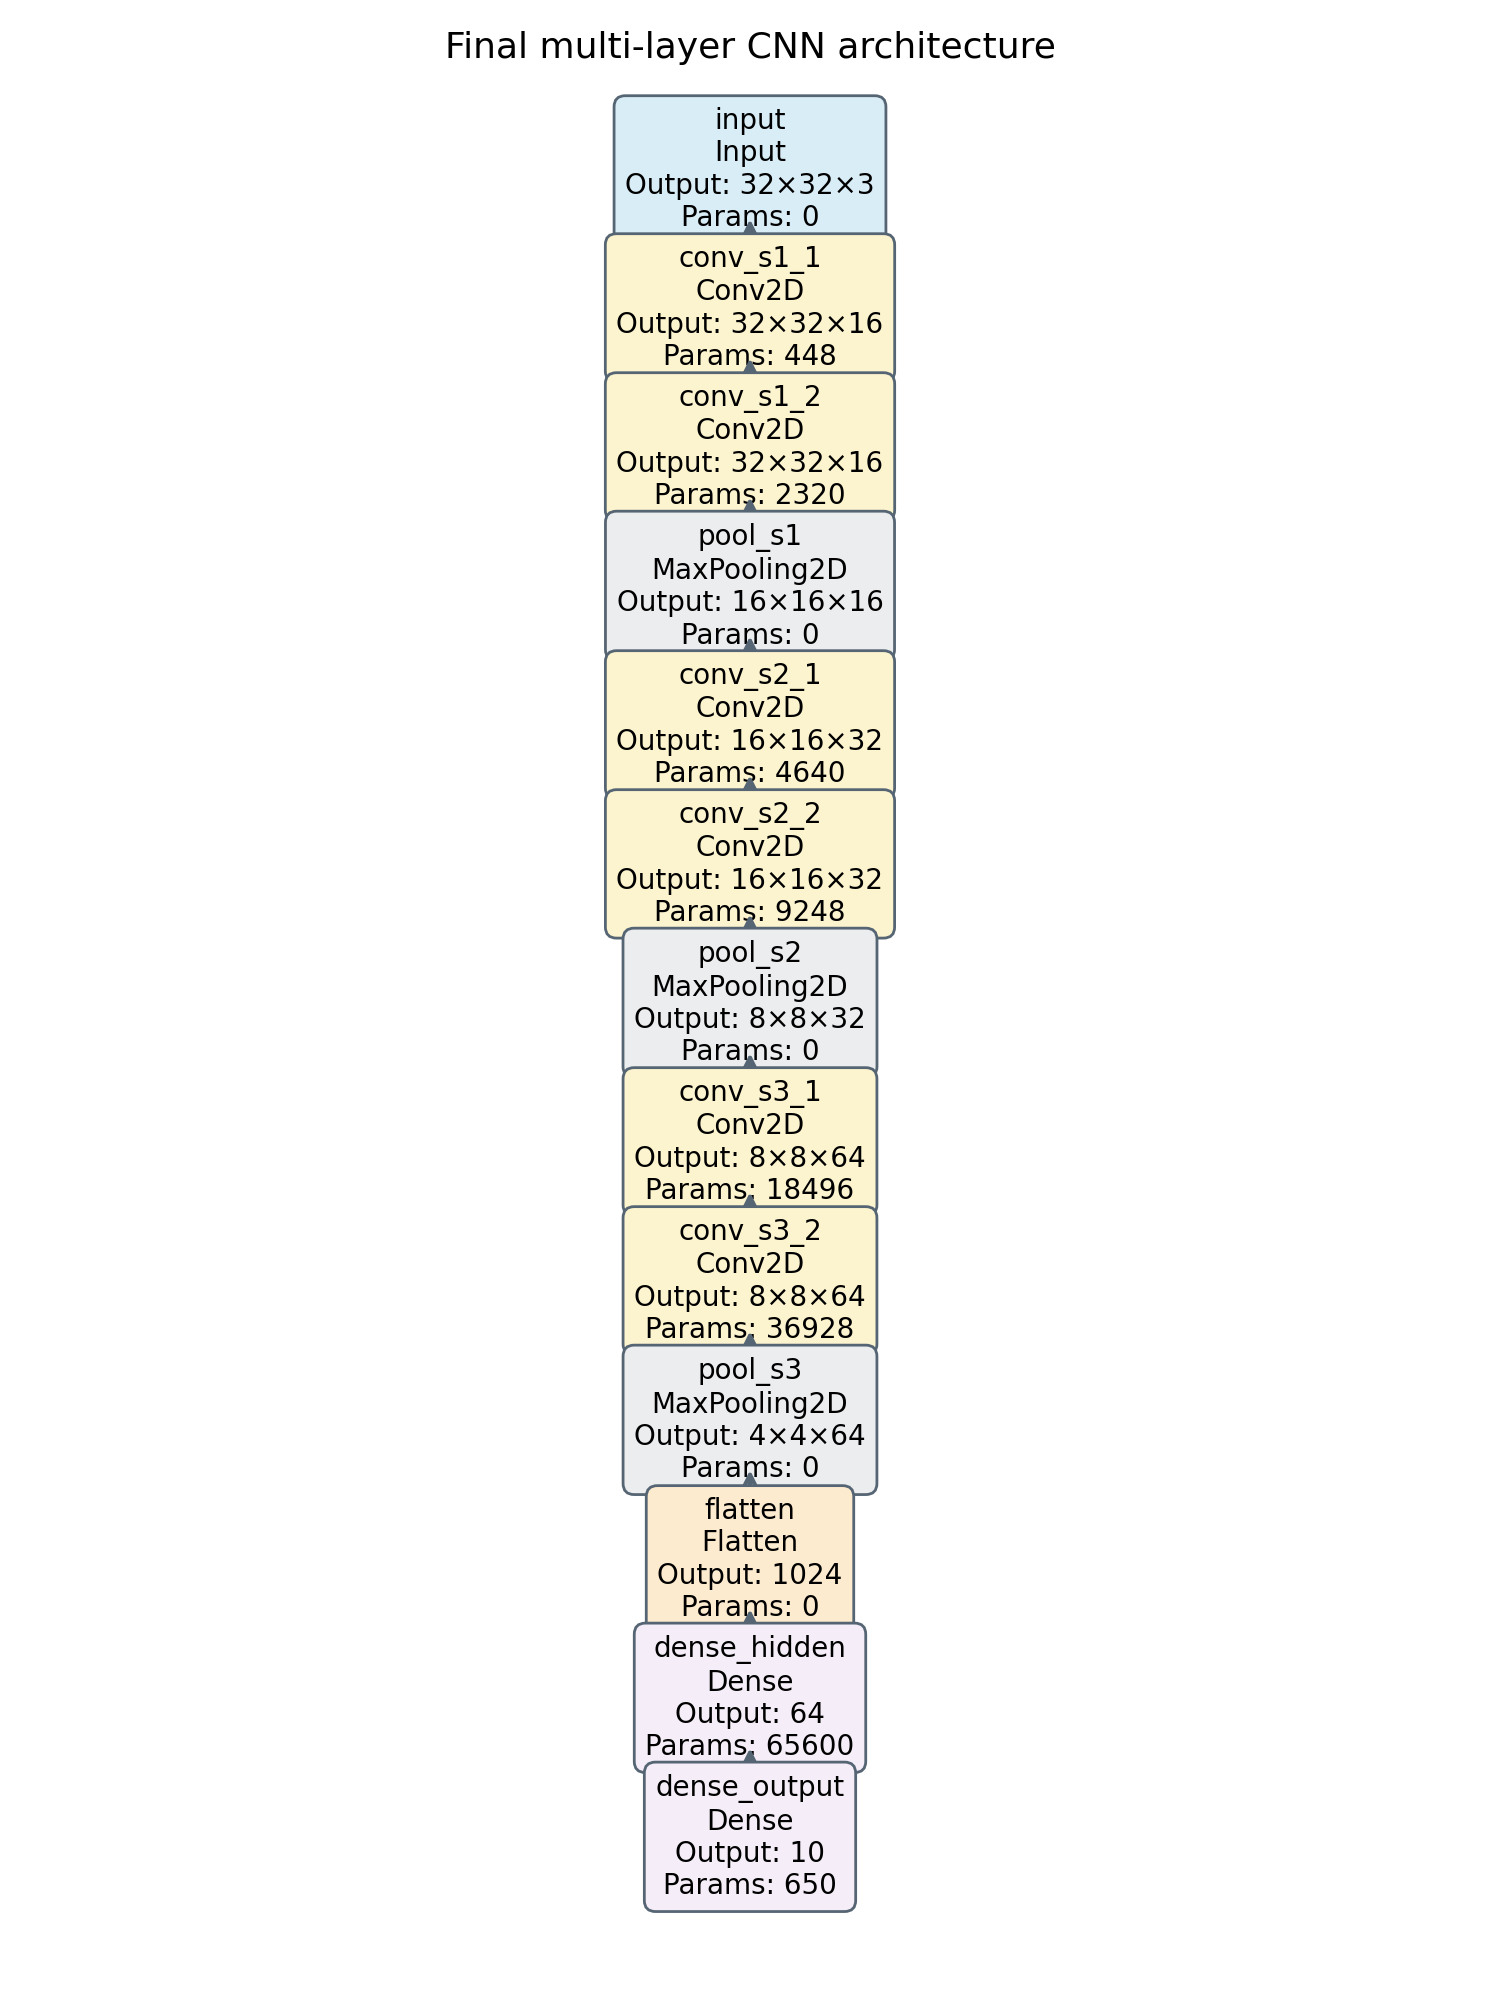
\includegraphics[width=0.8\linewidth]{imgs/section6_final_architecture.png}
\caption{Repr\'esentation graphique du mod\`ele final multi-couches. Le texte interne \`a la figure est laiss\'e en anglais pour garantir un rendu stable.}
\label{fig:section6_architecture}
\end{figure}

\begin{table}[htbp]
\centering
\caption{Hyperparam\`etres retenus pour le mod\`ele final $M3$.}
\label{tab:section6_hyperparameters}
\footnotesize
\begin{tabular}{|l|l|}
\hline
Backbone convolutionnel & $16$-$16$/pool $\rightarrow$ $32$-$32$/pool $\rightarrow$ $64$-$64$/pool \\
Kernel size & $(3,3)$ \\
Padding & \texttt{same} \\
Pool size & $(2,2)$ \\
Dense units & $64$ \\
Dropout apr\`es pooling & $0.25/0.25/0.25$ \\
Dropout avant dense & $0.5$ \\
P\'enalisation $L^2$ & $10^{-4}$ \\
Optimiseur & Adam \\
Learning rate & $10^{-3}$ \\
$\beta_1,\beta_2,\eta$ & $0.9, 0.999, 10^{-7}$ \\
Batch size & $32$ \\
Epochs & $12$ \\
\hline
\end{tabular}
\end{table}

Les courbes d\'apprentissage de la figure~\ref{fig:section6_curves} correspondent \`a un run repr\'esentatif du mod\`ele final avec la graine $42$. Elles montrent une progression r\'eguli\`ere de l'accuracy de validation jusqu\`a l'epoch $11$, o\`u celle-ci atteint $50.5\%$, avant un l\'eger recul \`a $49.2\%$ \`a l'epoch $12$. La \textit{val. loss} suit la m\^eme dynamique, avec un minimum \`a $1.4737$ \`a l'epoch $11$, puis une remont\'ee \`a $1.5332$ \`a l'epoch final. Cette inflexion signale un d\'ebut de sur-apprentissage, mais n'annule pas l'am\'elioration globale observ\'ee par rapport \`a la baseline.

\begin{figure}[htbp]
\centering
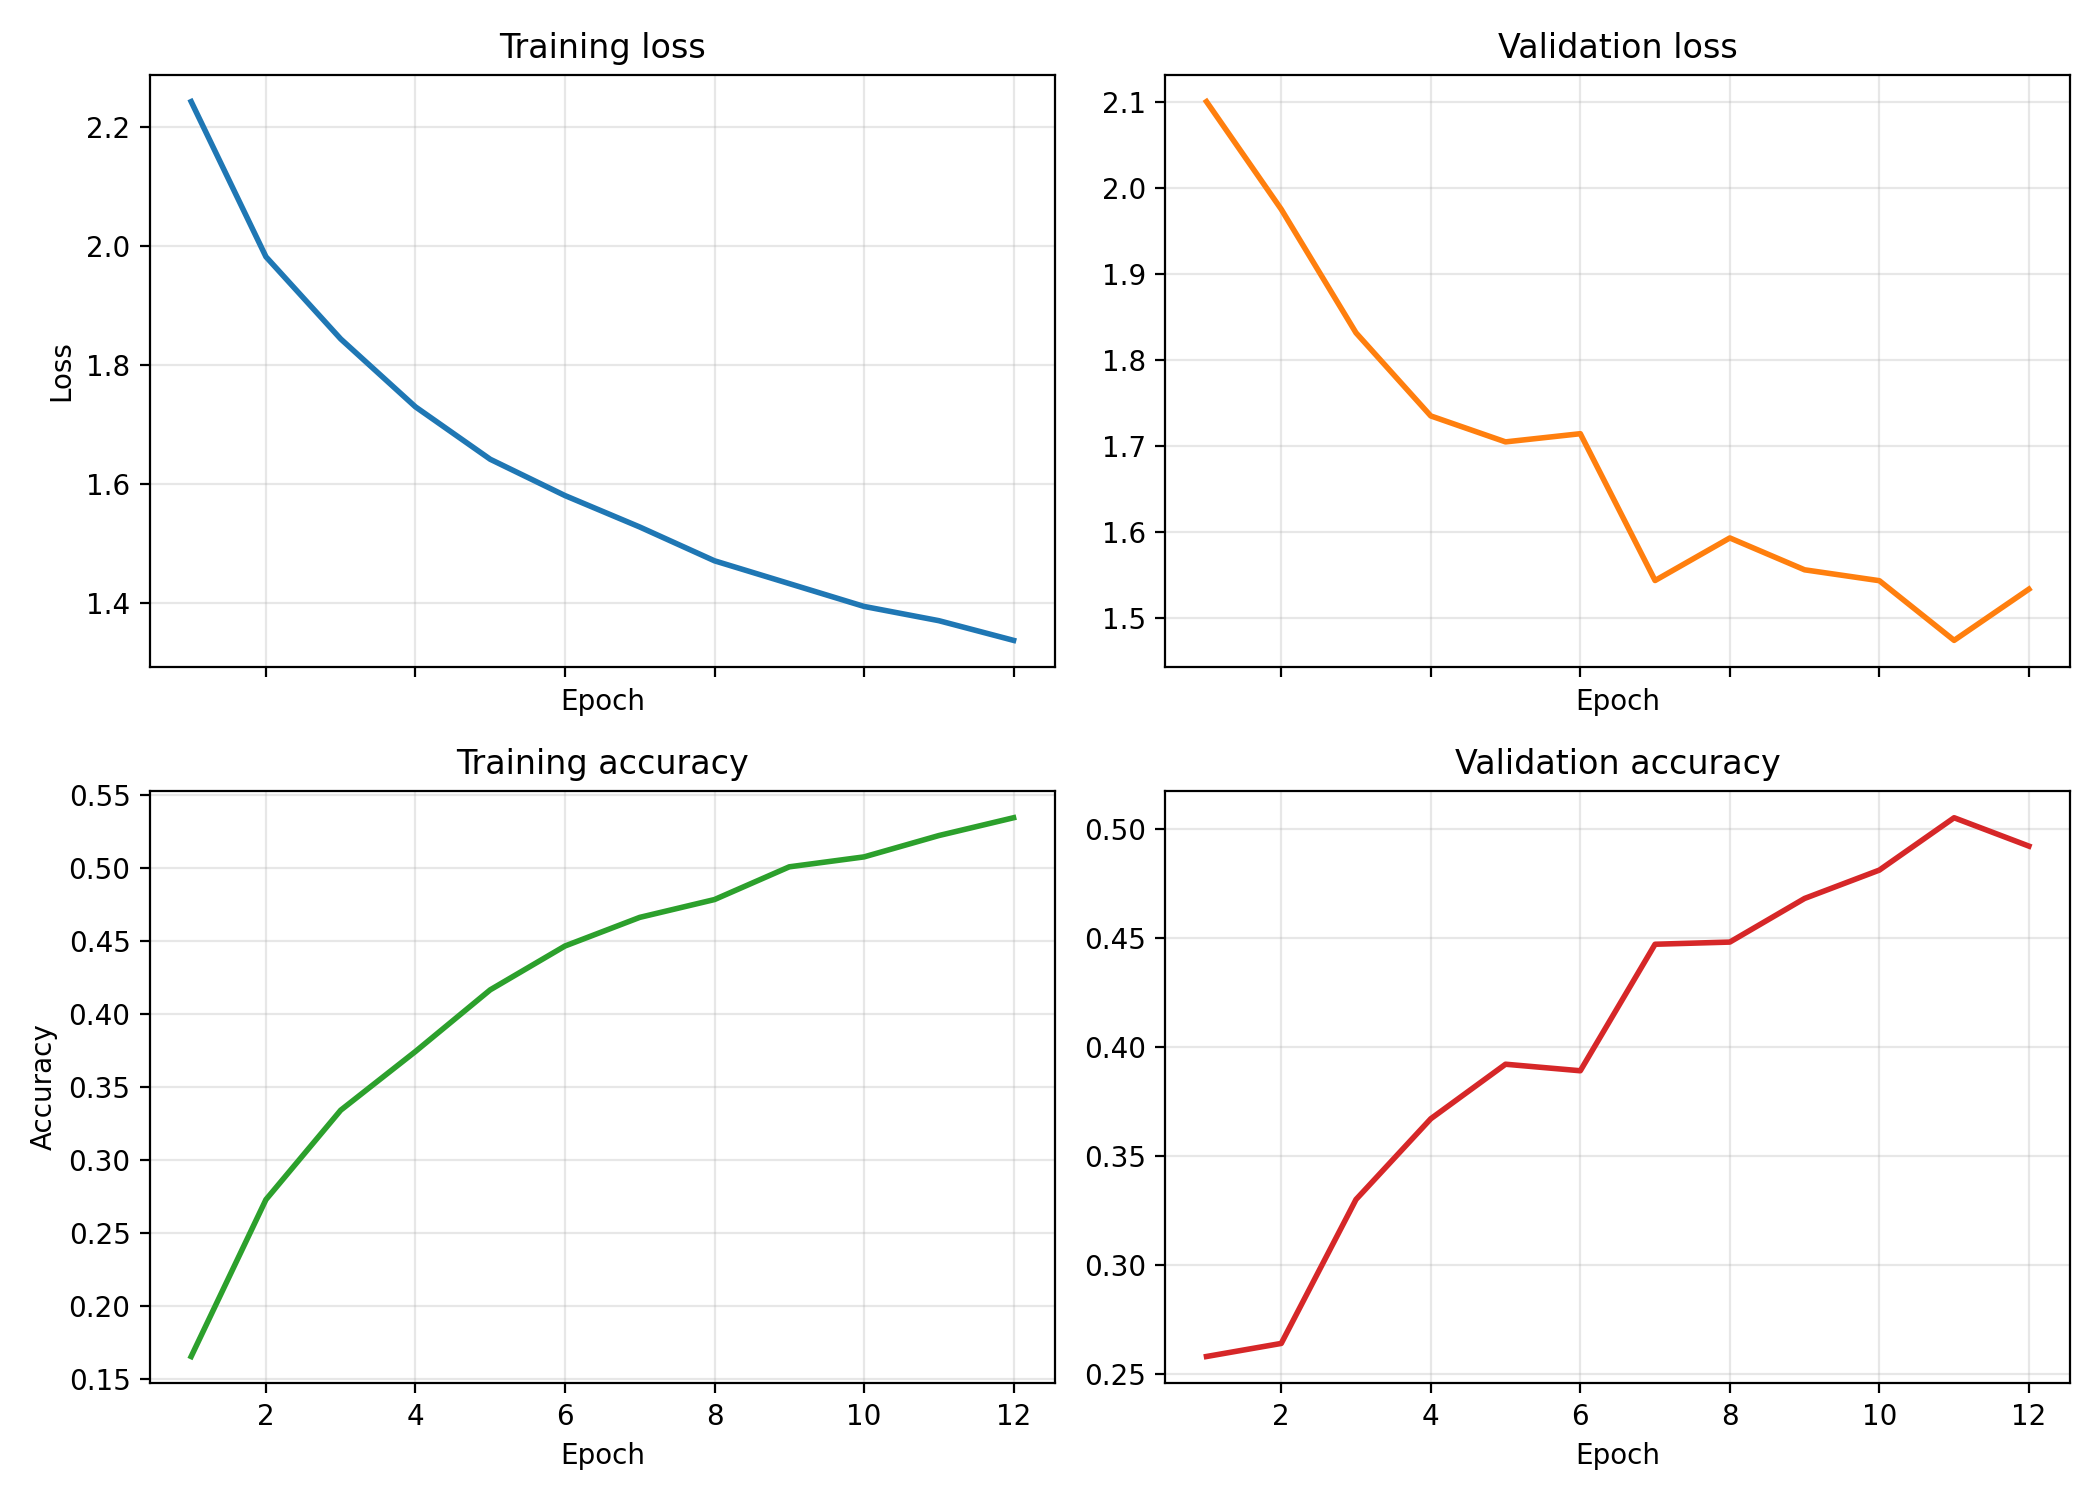
\includegraphics[width=\linewidth]{imgs/section6_final_curves.png}
\caption{Courbes d\'apprentissage du mod\`ele final $M3$ pour le run repr\'esentatif de graine $42$.}
\label{fig:section6_curves}
\end{figure}

Le mod\`ele final atteint sur l'ensemble de test r\'eduit une accuracy de $50.90\%$ et une loss de $1.5058$. Les matrices de confusion de la figure~\ref{fig:section6_confusion} montrent que les classes \textit{frog} ($83.81\%$), \textit{automobile} ($79.80\%$) et \textit{truck} ($72.13\%$) sont les mieux reconnues, tandis que \textit{cat} ($9.68\%$), \textit{bird} ($23.91\%$) et \textit{ship} ($28.92\%$) restent fragiles. Les plus fortes confusions hors diagonale concernent notamment \textit{cat} $\rightarrow$ \textit{dog}, \textit{deer} $\rightarrow$ \textit{frog}, ainsi que \textit{ship} $\rightarrow$ \textit{airplane} ou \textit{automobile}. L'approfondissement am\'eliore donc la s\'eparation de plusieurs classes, mais il ne supprime pas les ambigu\"it\'es visuelles les plus marqu\'ees.

\begin{figure}[htbp]
\centering
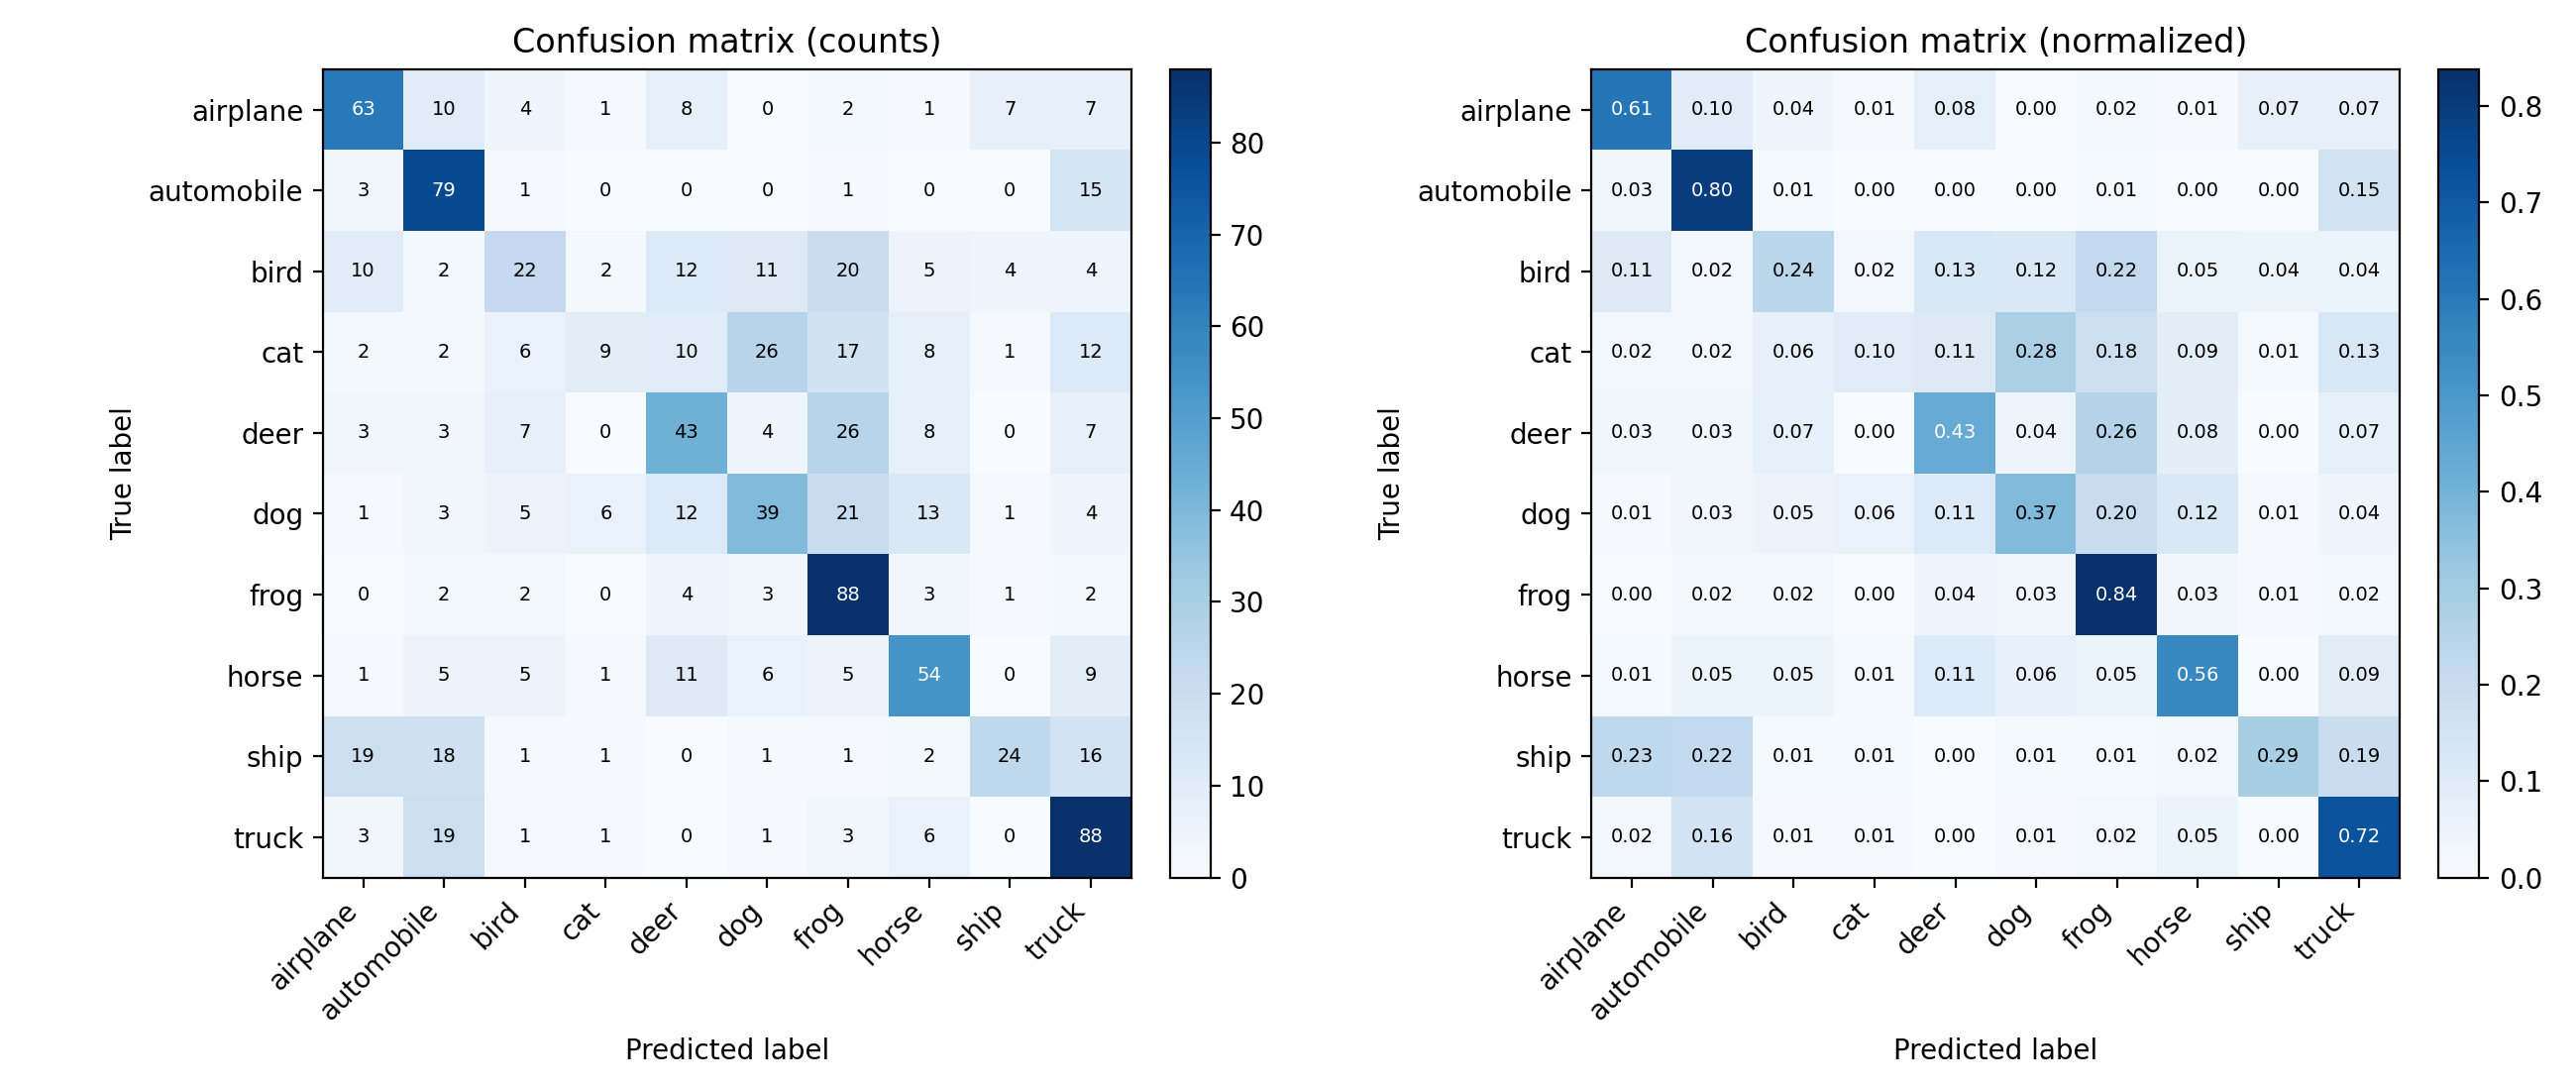
\includegraphics[width=\linewidth]{imgs/section6_final_confusion_matrices.png}
\caption{Matrices de confusion du mod\`ele final : version en effectifs et version normalis\'ee.}
\label{fig:section6_confusion}
\end{figure}

\subsection{Discussion critique : avantages et limites}
L'approfondissement du r\'eseau apporte un gain mesurable et coh\'erent avec le cadre th\'eorique du cours. En empilant plusieurs couches convolutionnelles, le mod\`ele retient des caract\'eristiques plus hi\'erarchiques et voit son champ r\'ecepteur effectif s'agrandir au fil des couches. Cette structuration se traduit ici par une am\'elioration de l'accuracy de validation de $42.30\%$ \`a $50.80\%$ entre $M0$ et $M3$, sans explosion du nombre total de param\`etres. Le gain ne provient donc pas d'une seule augmentation massive de la taille du classifieur dense, mais bien d'une meilleure exploitation de la partie convolutionnelle.

La comparaison entre $M2$ et $M3$ montre en outre que la profondeur seule ne suffit pas. \`A backbone identique, la r\'egularisation explicite de $M3$ am\'eliore nettement la validation et abaisse la \textit{val. loss}. Le \textit{dropout} et la p\'enalisation $L^2$ jouent donc ici le r\^ole attendu : ils limitent la co-adaptation des neurones et contraignent la norme des poids, ce qui devient utile sur un sous-ensemble d'apprentissage aussi restreint.

Les limites du mod\`ele restent n\'eanmoins visibles. D'abord, le co\^ut calculatoire augmente sensiblement : $M3$ exige pr\`es de trois fois plus de temps par epoch que la baseline. Ensuite, la performance absolue demeure mod\'er\'ee sur le test r\'eduit, avec $50.90\%$ d\'accuracy, ce qui montre que la profondeur ne compense ni la petite taille du corpus d\'entra\^inement, ni les ambigu\"it\'es visuelles fortes entre certaines classes. Enfin, les courbes du run repr\'esentatif montrent un d\'ebut de sur-apprentissage en fin d\'entra\^inement, ce qui sugg\`ere que le budget de $12$ epochs reste proche de la limite utile pour cette architecture et ce protocole.

Sous le protocole retenu, l'ajout de profondeur appara\^it donc justifi\'e lorsque la priorit\'e est la pr\'ecision de validation. Le gain de $8.5$ points par rapport \`a la baseline est substantiel, et il s'accompagne d'un meilleur minimum de \textit{val. loss} ainsi que d'une meilleure s\'eparation de plusieurs classes. En revanche, ce raffinement n'a rien d'universel : son int\'er\^et resterait \`a reconsid\'erer si la contrainte principale devenait le temps de calcul plut\^ot que la performance finale.

\section{Sur-apprentissage}

\subsection{Identification du sur-apprentissage sur les courbes de co\^ut}
Dans le cadre de l'apprentissage supervis\'e, le sur-apprentissage d\'esigne une situation dans laquelle l'optimisation de la loss empirique sur l'ensemble d'apprentissage se poursuit alors que la qualit\'e de g\'en\'eralisation se d\'egrade sur l'ensemble de validation. Si l'on note $L_{\mathrm{app}}^{(t)}$ et $L_{\mathrm{val}}^{(t)}$ les co\^uts observ\'es \`a l'epoch $t$ sur les ensembles d'apprentissage et de validation, le signe caract\'eristique du sur-apprentissage est la poursuite de la d\'ecroissance de $L_{\mathrm{app}}^{(t)}$ alors que $L_{\mathrm{val}}^{(t)}$ recommence \`a cro\^itre apr\`es un minimum. Cette divergence traduit une am\'elioration de l'ajustement aux donn\'ees vues sans gain de g\'en\'eralisation sur les donn\'ees non utilis\'ees pour la mise \`a jour des poids \cite{manzanera_classification_apprentissage,poly_chap4_classifml}.

Pour quantifier ce ph\'enom\`ene, la pr\'esente section retient l'indicateur
\begin{equation}
\Delta_{\mathrm{sur}}
=
L_{\mathrm{val}}^{(T)}
-
\min_{1 \leq t \leq T} L_{\mathrm{val}}^{(t)},
\label{eq:section7_overfit_increase}
\end{equation}
o\`u $T$ d\'esigne l'epoch final du protocole. Une valeur positive de $\Delta_{\mathrm{sur}}$ indique que la loss de validation finale est sup\'erieure \`a son meilleur niveau atteint pendant l'apprentissage. Plus cette quantit\'e est grande, plus la d\'egradation de g\'en\'eralisation en fin d'entra\^inement est marqu\'ee. Le ph\'enom\`ene est d'autant plus probable que la capacit\'e du mod\`ele est \'elev\'ee, que le corpus d'apprentissage est r\'eduit et que la dur\'ee d'entra\^inement est prolong\'ee sans r\'egularisation explicite \cite{poly_chap4_classifml}.

\subsection{Exemple issu du workflow de la Section~6}
La Section~6 fournit d\'ej\`a un exemple exploitable sans introduire de nouvelle architecture. Le \textit{screening} du mod\`ele $M2$ (\textit{three-stage CNN} non r\'egularis\'e), ex\'ecut\'e avec la graine $42$ pendant $10$ epochs, pr\'esente un comportement de sur-apprentissage net. La figure~\ref{fig:section7_overfitting_example} montre que la loss d'apprentissage d\'ecro\^it presque monotoniquement, de $2.0646$ \`a $0.5822$, tandis que la loss de validation atteint un minimum de $1.6178$ \`a l'epoch $4$ avant de remonter jusqu'\`a $2.5590$ \`a l'epoch $10$. Il en r\'esulte
\begin{equation}
\Delta_{\mathrm{sur}} = 2.5590 - 1.6178 = 0.9412.
\end{equation}

Le m\^eme diagnostic appara\^it sur les accuracies : l'accuracy d'apprentissage finale atteint $78.96\%$, alors que l'accuracy finale de validation reste \`a $43.60\%$, soit un \'ecart de $35.36$ points. La meilleure accuracy de validation, $48.20\%$, est d'ailleurs obtenue avant la fin de l'entra\^inement. Ce run constitue donc un exemple pertinent pour illustrer la distinction entre optimisation r\'eussie de l'objectif d'apprentissage et d\'egradation de la g\'en\'eralisation.

\begin{figure}[htbp]
\centering
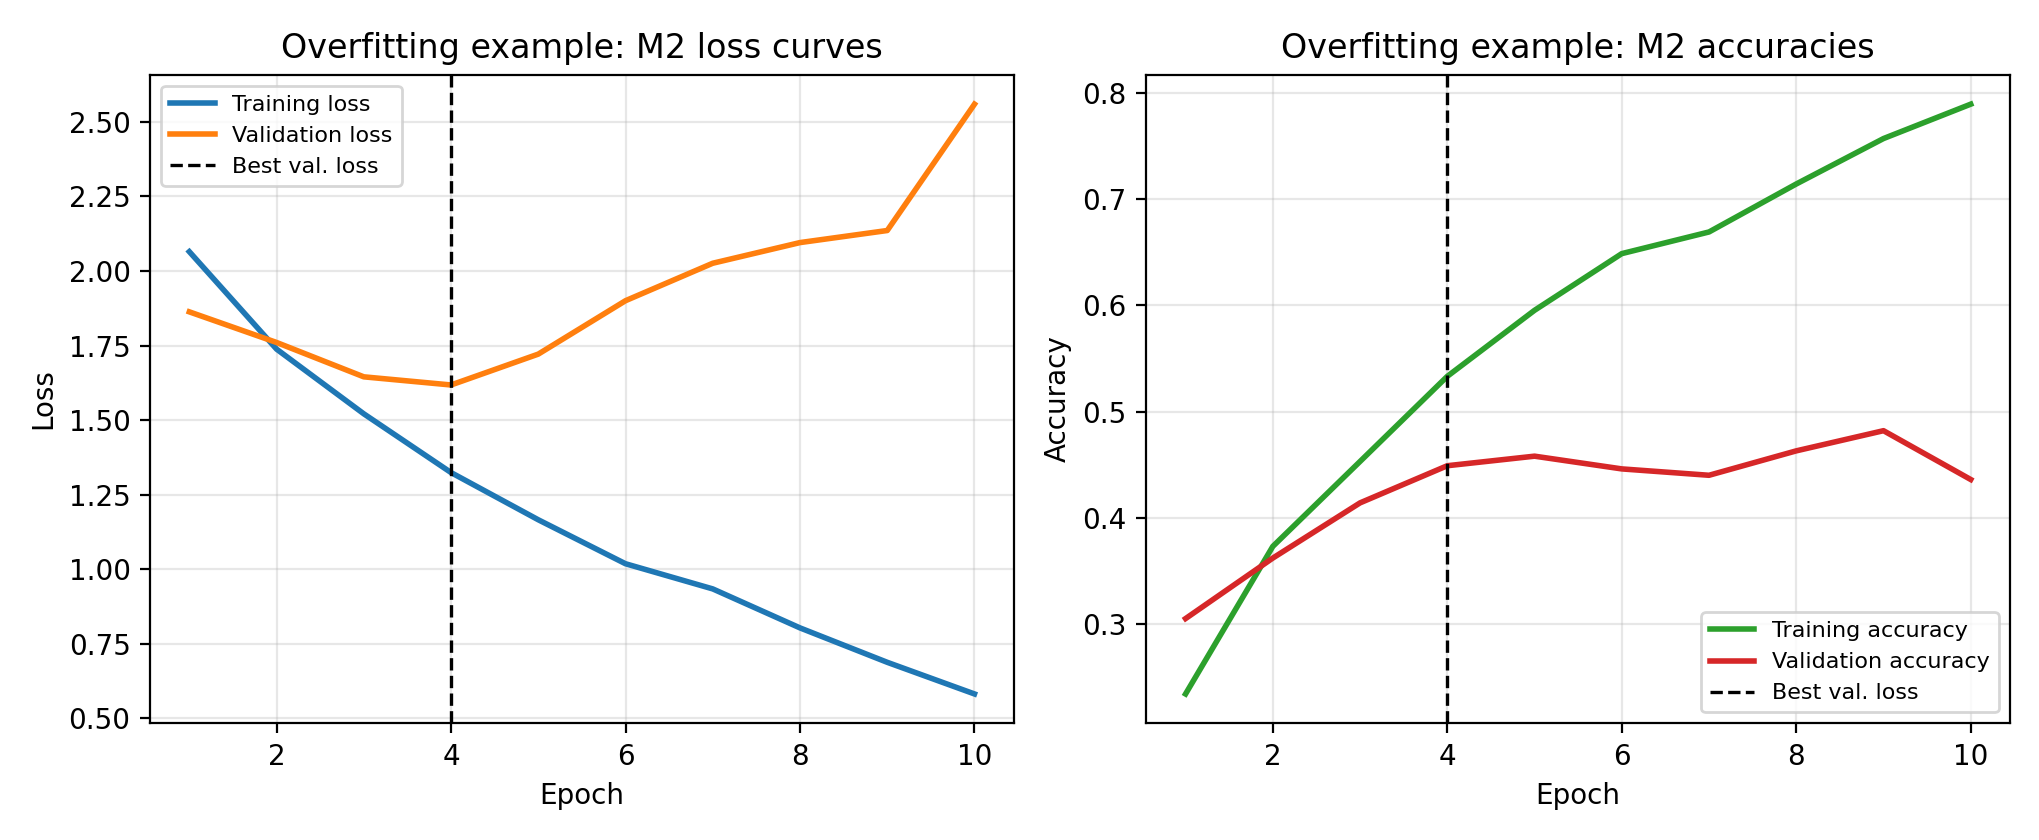
\includegraphics[width=\linewidth]{imgs/section7_overfitting_example.png}
\caption{Exemple de sur-apprentissage r\'eutilis\'e depuis la Section~6 : mod\`ele $M2$, graine $42$, $10$ epochs. Le texte interne \`a la figure est laiss\'e en anglais pour garantir un rendu stable.}
\label{fig:section7_overfitting_example}
\end{figure}

\subsection{Effet de m\'ecanismes de r\'egularisation}
Afin d'\'etudier des m\'ecanismes susceptibles de r\'eduire ce ph\'enom\`ene, une campagne contr\^ol\'ee a \'et\'e men\'ee sur le m\^eme backbone profond que celui de $M2$. Le protocole reste identique \`a celui de la Section~6 : m\^eme split CIFAR-10 r\'eduit ($5000/1000/1000$), m\^eme standardisation image par image, Adam avec $(\epsilon,\beta_1,\beta_2,\eta)=(10^{-3},0.9,0.999,10^{-7})$, \textit{batch size} $32$, \texttt{shuffle=True}, graines $42$ et $314$, et budget fix\'e \`a $15$ epochs. Quatre variantes ont \'et\'e compar\'ees :
\begin{itemize}
\item $R0$ : backbone $M2$ sans r\'egularisation explicite ;
\item $R1$ : backbone $M2$ avec \textit{dropout} ($0.25$ apr\`es chaque \textit{pooling}, $0.5$ avant la couche dense) ;
\item $R2$ : backbone $M2$ avec seule p\'enalisation $L^2$ de coefficient $10^{-4}$ ;
\item $R3$ : mod\`ele $M3$ de la Section~6, combinant \textit{dropout} et p\'enalisation $L^2$.
\end{itemize}

Ces choix correspondent \`a deux m\'ecanismes de r\'egularisation explicitement discut\'es dans le cours. Le \textit{dropout} limite la co-adaptation des neurones en supprimant al\'eatoirement une partie des activations pendant l'apprentissage, alors que la p\'enalisation $L^2$ contraint la norme des poids et d\'ecourage des solutions trop fortement ajust\'ees au corpus d'apprentissage \cite{manzanera_classification_apprentissage,poly_chap4_classifml}. La figure~\ref{fig:section7_regularization_comparison} et le tableau~\ref{tab:section7_regularization} r\'esument les effets observ\'es.

\begin{table*}[htbp]
\centering
\caption{Comparaison des m\'ecanismes de r\'egularisation sur le backbone profond de la Section~6. Le symbole $\pm$ d\'esigne l'\'ecart-type empirique sur les deux graines.}
\label{tab:section7_regularization}
\small
\begin{tabular}{|c|l|c|c|c|c|}
\hline
Variante & M\'ecanisme & Accuracy finale val. (\%) & Min. val. loss & $\Delta_{\mathrm{sur}}$ & \'Ecart final train-val (pts) \\
\hline
$R0$ & aucune & $47.30 \pm 2.00$ & $1.6192 \pm 0.0014$ & $1.3744 \pm 0.0740$ & $43.87 \pm 1.37$ \\
$R1$ & dropout & $53.90 \pm 1.80$ & $1.2743 \pm 0.0636$ & $0.0211 \pm 0.0152$ & $5.58 \pm 0.34$ \\
$R2$ & $L^2$ seul & $48.55 \pm 2.05$ & $1.6630 \pm 0.0763$ & $1.8604 \pm 0.0397$ & $41.79 \pm 0.13$ \\
$R3$ & dropout + $L^2$ & $55.50 \pm 1.10$ & $1.3410 \pm 0.0246$ & $0.0000 \pm 0.0000$ & $3.70 \pm 0.38$ \\
\hline
\end{tabular}
\end{table*}

\begin{figure}[htbp]
\centering
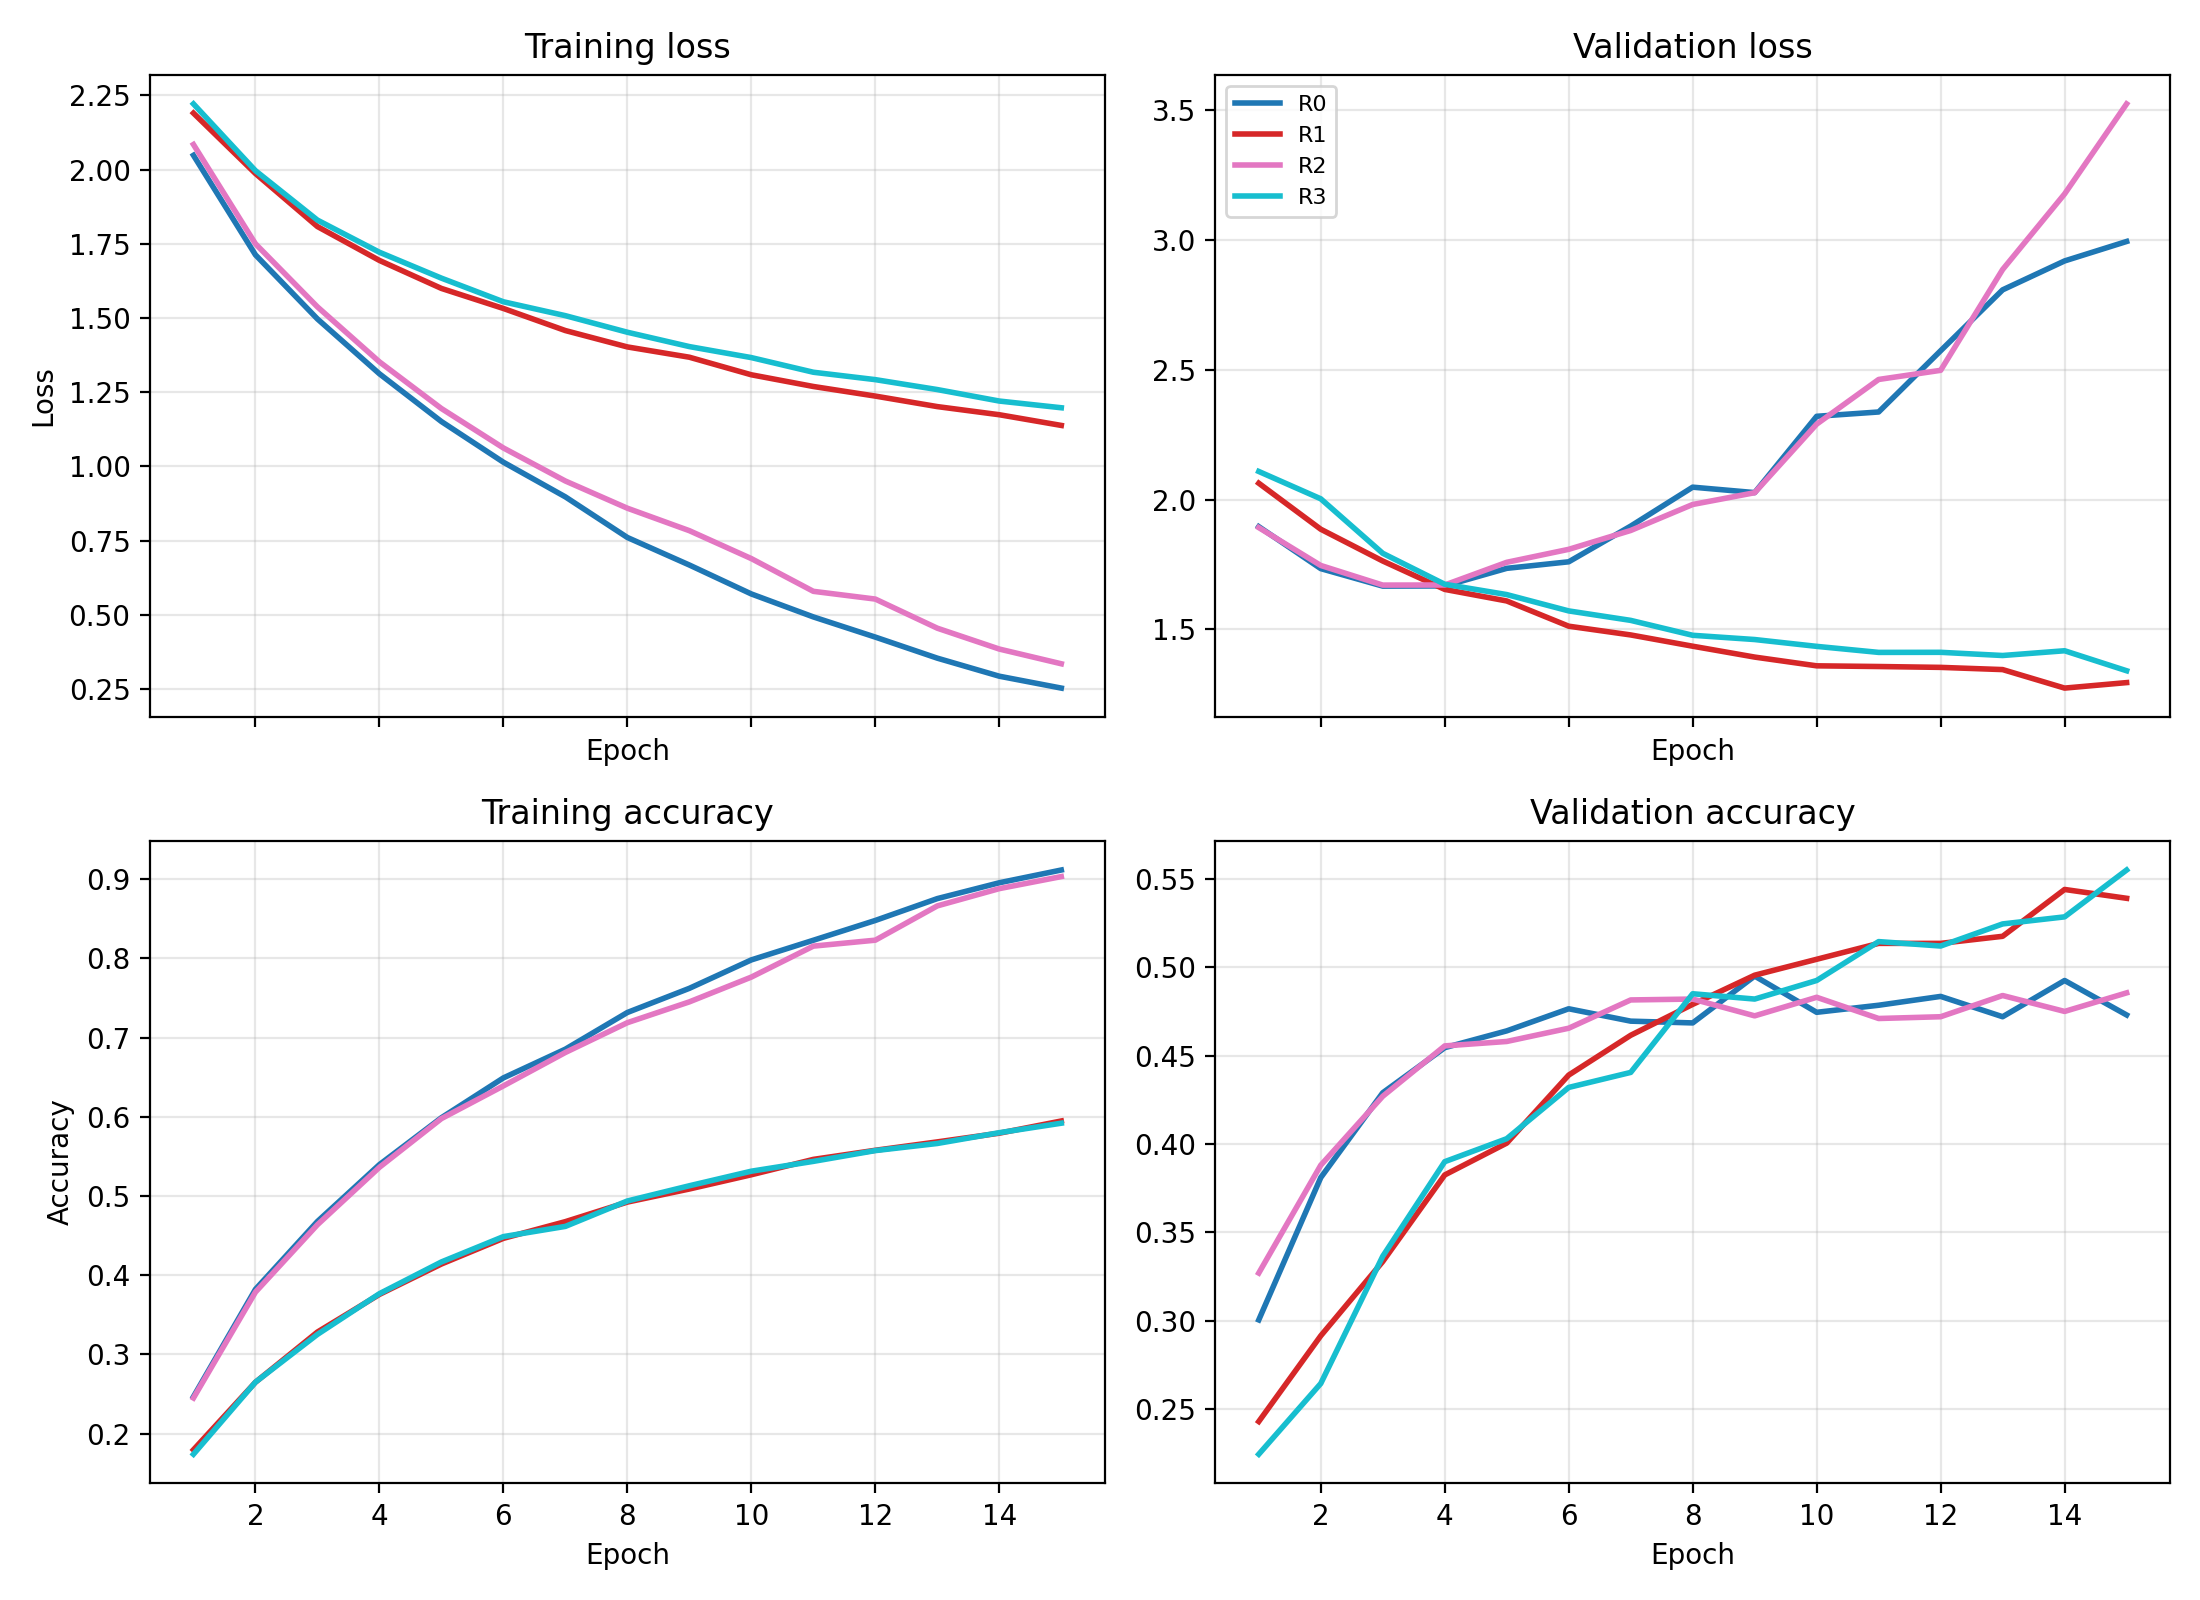
\includegraphics[width=\linewidth]{imgs/section7_regularization_comparison.png}
\caption{Comparaison des courbes moyennes d'apprentissage et de validation pour les variantes $R0$ \`a $R3$. Le texte interne \`a la figure est laiss\'e en anglais pour garantir un rendu stable.}
\label{fig:section7_regularization_comparison}
\end{figure}

\begin{figure}[htbp]
\centering
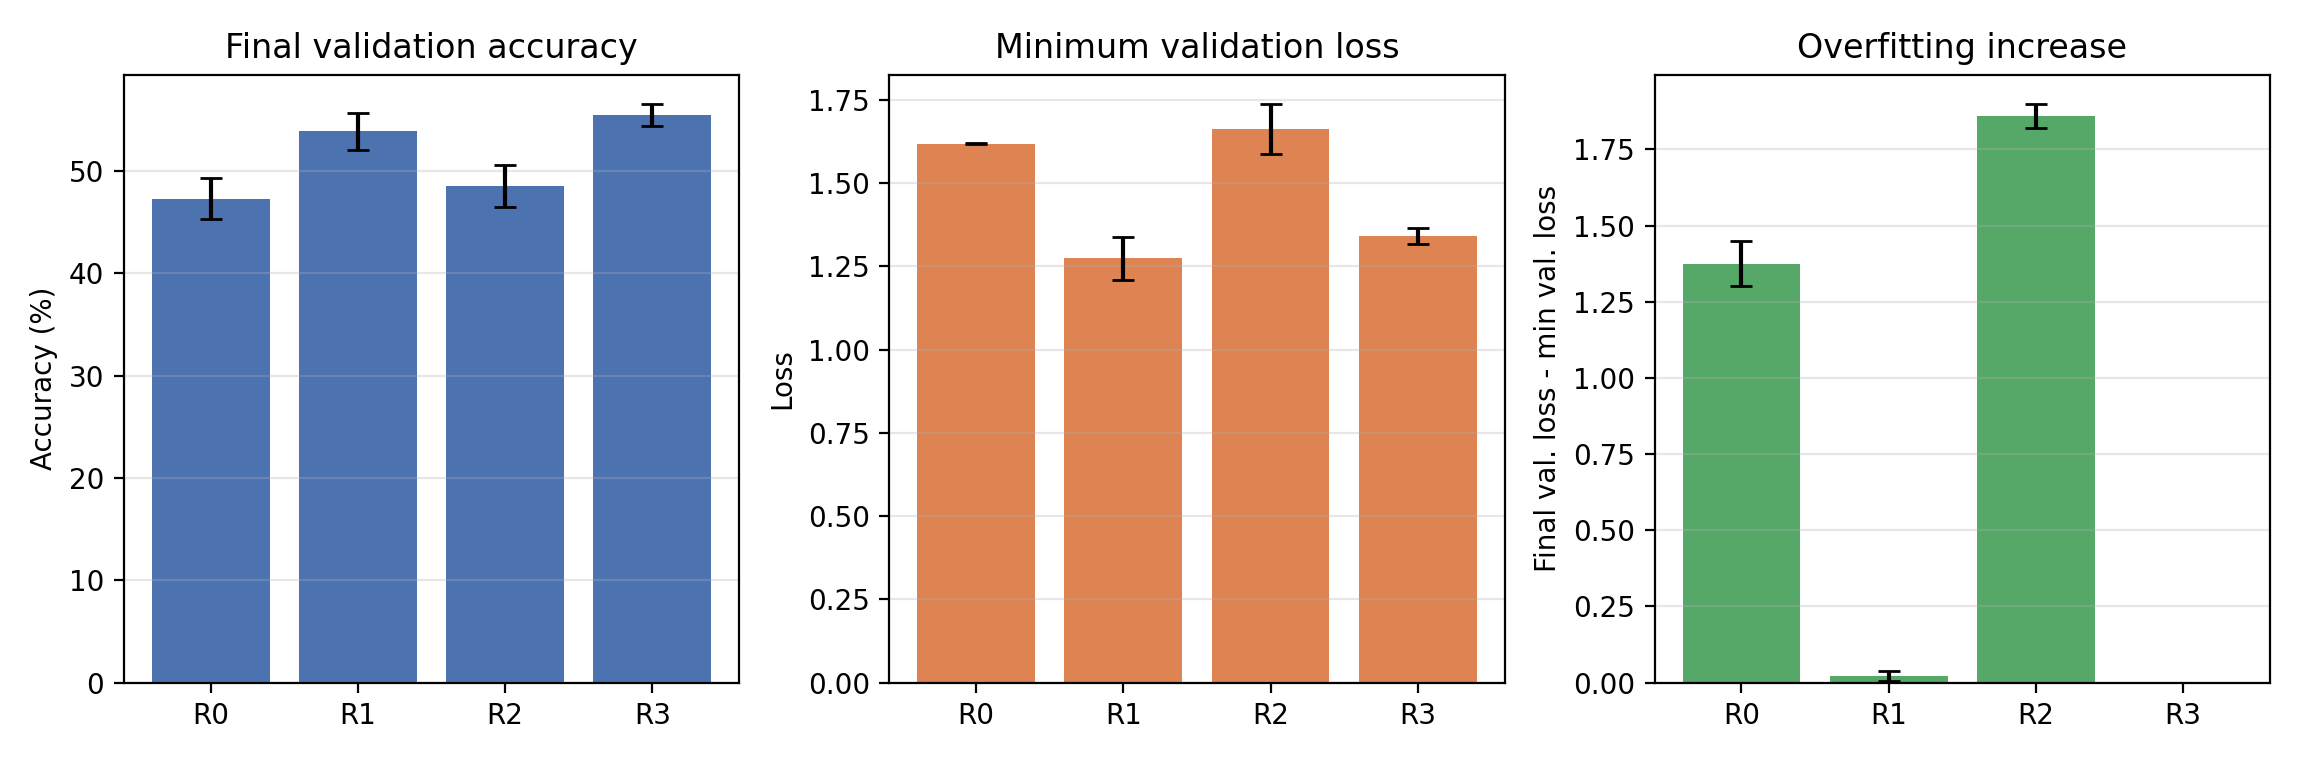
\includegraphics[width=\linewidth]{imgs/section7_regularization_summary.png}
\caption{Synth\`ese graphique des effets observ\'es sur l'accuracy finale de validation, le minimum de \textit{val. loss} et l'indicateur $\Delta_{\mathrm{sur}}$.}
\label{fig:section7_regularization_summary}
\end{figure}

Le comportement de $R0$ confirme le diagnostic initial : la loss d'apprentissage continue de d\'ecro\^itre jusqu'\`a $0.2536$, alors que la loss de validation remonte jusqu'\`a $2.9937$ apr\`es un minimum moyen de $1.6192$. L'indicateur moyen $\Delta_{\mathrm{sur}}=1.3744$ et l'\'ecart final train-val de $43.87$ points t\'emoignent d'une g\'en\'eralisation fortement d\'egrad\'ee. L'ajout du seul \textit{dropout} dans $R1$ modifie radicalement cette dynamique : la loss de validation reste presque monotone jusqu'\`a l'epoch $14$, et $\Delta_{\mathrm{sur}}$ chute \`a $0.0211$. Cette r\'egularisation ralentit l'optimisation sur l'ensemble d'apprentissage, puisque l'accuracy finale train n'est plus que de $59.48\%$, mais elle am\'eliore nettement la validation, avec $53.90\%$ d'accuracy finale et le meilleur minimum moyen de \textit{val. loss} ($1.2743$).

La p\'enalisation $L^2$ seule, test\'ee dans $R2$, ne produit pas le m\^eme effet sous ce protocole. L'accuracy finale de validation, $48.55\%$, reste proche de $R0$, tandis que $\Delta_{\mathrm{sur}}$ atteint $1.8604$, soit une d\'egradation encore plus forte que pour la baseline non r\'egularis\'ee. Cette observation indique que, dans ce cadre exp\'erimental, le coefficient $10^{-4}$ ne suffit pas \`a contenir le sur-apprentissage du backbone profond lorsqu'il est utilis\'e sans \textit{dropout}. Enfin, la combinaison des deux m\'ecanismes dans $R3$ donne le meilleur compromis global : l'accuracy finale de validation atteint $55.50\%$, l'\'ecart train-val tombe \`a $3.70$ points et la loss de validation continue \`a d\'ecro\^itre jusqu'\`a l'epoch final, ce qui conduit \`a $\Delta_{\mathrm{sur}}=0$ sur le budget fix\'e \`a $15$ epochs.

\subsection{Discussion comparative}
Les r\'esultats montrent que la lecture des courbes de co\^ut fournit un crit\`ere de diagnostic plus fiable que la seule observation de l'accuracy finale. Dans les variantes non suffisamment r\'egularis\'ees, l'optimisation du co\^ut d'apprentissage se poursuit alors que la loss de validation se d\'egrade, ce qui signale un apprentissage trop sp\'ecifique aux donn\'ees vues. Ce comportement appara\^it tr\`es clairement pour $M2$ dans l'exemple issu de la Section~6, puis pour $R0$ et $R2$ dans la comparaison contr\^ol\'ee.

La comparaison met aussi en \'evidence que tous les m\'ecanismes de r\'egularisation ne se valent pas dans le protocole retenu. Le \textit{dropout} r\'eduit fortement la co-adaptation et am\'eliore d\'ej\`a nettement la g\'en\'eralisation lorsqu'il est utilis\'e seul. La p\'enalisation $L^2$ de coefficient $10^{-4}$, en revanche, ne suffit pas \`a elle seule \`a stabiliser la validation pour ce backbone et ce budget d'entra\^inement. La combinaison des deux m\'ecanismes fournit finalement le meilleur compromis entre limitation du sur-apprentissage et performance finale, en prolongeant la d\'ecroissance de la loss de validation jusqu'\`a la fin du protocole.

Ces observations restent coh\'erentes avec la Section~6. L'augmentation de profondeur am\'eliore la capacit\'e de repr\'esentation du mod\`ele, mais elle accro\^it aussi le risque de sur-ajustement sur un sous-ensemble d'apprentissage limit\'e \`a $5000$ images. Dans ce contexte, l'introduction de \textit{dropout} et d'une p\'enalisation $L^2$ ne constitue pas un raffinement optionnel, mais une condition importante pour exploiter utilement la capacit\'e suppl\'ementaire du backbone profond. Une strat\'egie telle que l'\textit{early stopping} pourrait encore \^etre mobilis\'ee pour arr\^eter l'entra\^inement au voisinage du minimum de validation, mais elle n'a pas \'et\'e retenue ici afin de conserver un budget d'epochs identique pour toutes les variantes compar\'ees.

\section{Cartes d'activation}

\subsection{Interpr\'etation des cartes d'activation de la premi\`ere couche}
Pour une image d'entr\'ee $X$ et une couche convolutionnelle $l$, la carte d'activation du canal $m$ est la r\'eponse spatiale
\begin{equation}
A_m^{(l)}(X)=\phi\!\left(z^{(l)}_{:,:,m}(X)\right),
\end{equation}
c'est-\`a-dire la sortie du filtre $m$ apr\`es convolution et non-lin\'earit\'e. Il convient donc de distinguer les filtres appris $K^{(l)}_{u,v,c,m}$, qui constituent les poids adaptables du r\'eseau, des cartes d'activation, qui d\'ependent \`a la fois de ces poids et de l'image analys\'ee. Les couches successives composent ainsi une banque de filtres locaux et des transformations non lin\'eaires hi\'erarchiques, conform\'ement au cadre pr\'esent\'e dans le cours \cite{lecun_convolutional_networks,manzanera_classification_apprentissage,poly_chap4_classifml}.

La pr\'esente section r\'eutilise le mod\`ele profond r\'egularis\'e $M3/R3$ retenu aux Sections~6 et~7. Le run de r\'ef\'erence correspond \`a une architecture \`a trois \'etages convolutionnels entra\^in\'ee pendant $15$ epochs avec Adam sur le m\^eme split CIFAR-10 r\'eduit et la m\^eme standardisation image par image ; il atteint $53.70\%$ d'accuracy sur l'ensemble de test, pour une accuracy finale de validation de $53.80\%$ et un maximum de validation de $54.10\%$. Pour garantir une lecture stable, le rapport retient comme image principale un exemple de la classe \textit{truck}, correctement class\'e avec une confiance de $0.9933$.

La figure~\ref{fig:section8_first_layer} pr\'esente les $16$ cartes produites par la premi\`ere couche convolutionnelle \texttt{conv\_s1\_1}, de taille $32\times 32\times 16$. Plusieurs canaux r\'eagissent nettement aux transitions de luminance entre la carrosserie du camion, l'horizon et la chauss\'ee, tandis que d'autres soulignent davantage les contrastes chromatiques entre le ciel bleu, les zones gris-beige du v\'ehicule et l'arri\`ere-plan. Une mesure objective fond\'ee sur des corr\'elations avec des proxys simples confirme cette lecture prudente : les canaux $1$, $14$ et $12$ sont les plus corr\'el\'es \`a la norme du gradient, tandis que les canaux $10$, $7$ et $8$ sont les plus sensibles au contraste chromatique. La moyenne du taux d'activations positives vaut $0.464$ et l'entropie spatiale normalis\'ee moyenne $0.847$, ce qui indique des cartes encore denses et localement interpr\'etables, coh\'erentes avec un premier niveau de d\'etection de contours, de contraste local et de motifs simples.

\begin{figure}[htbp]
\centering
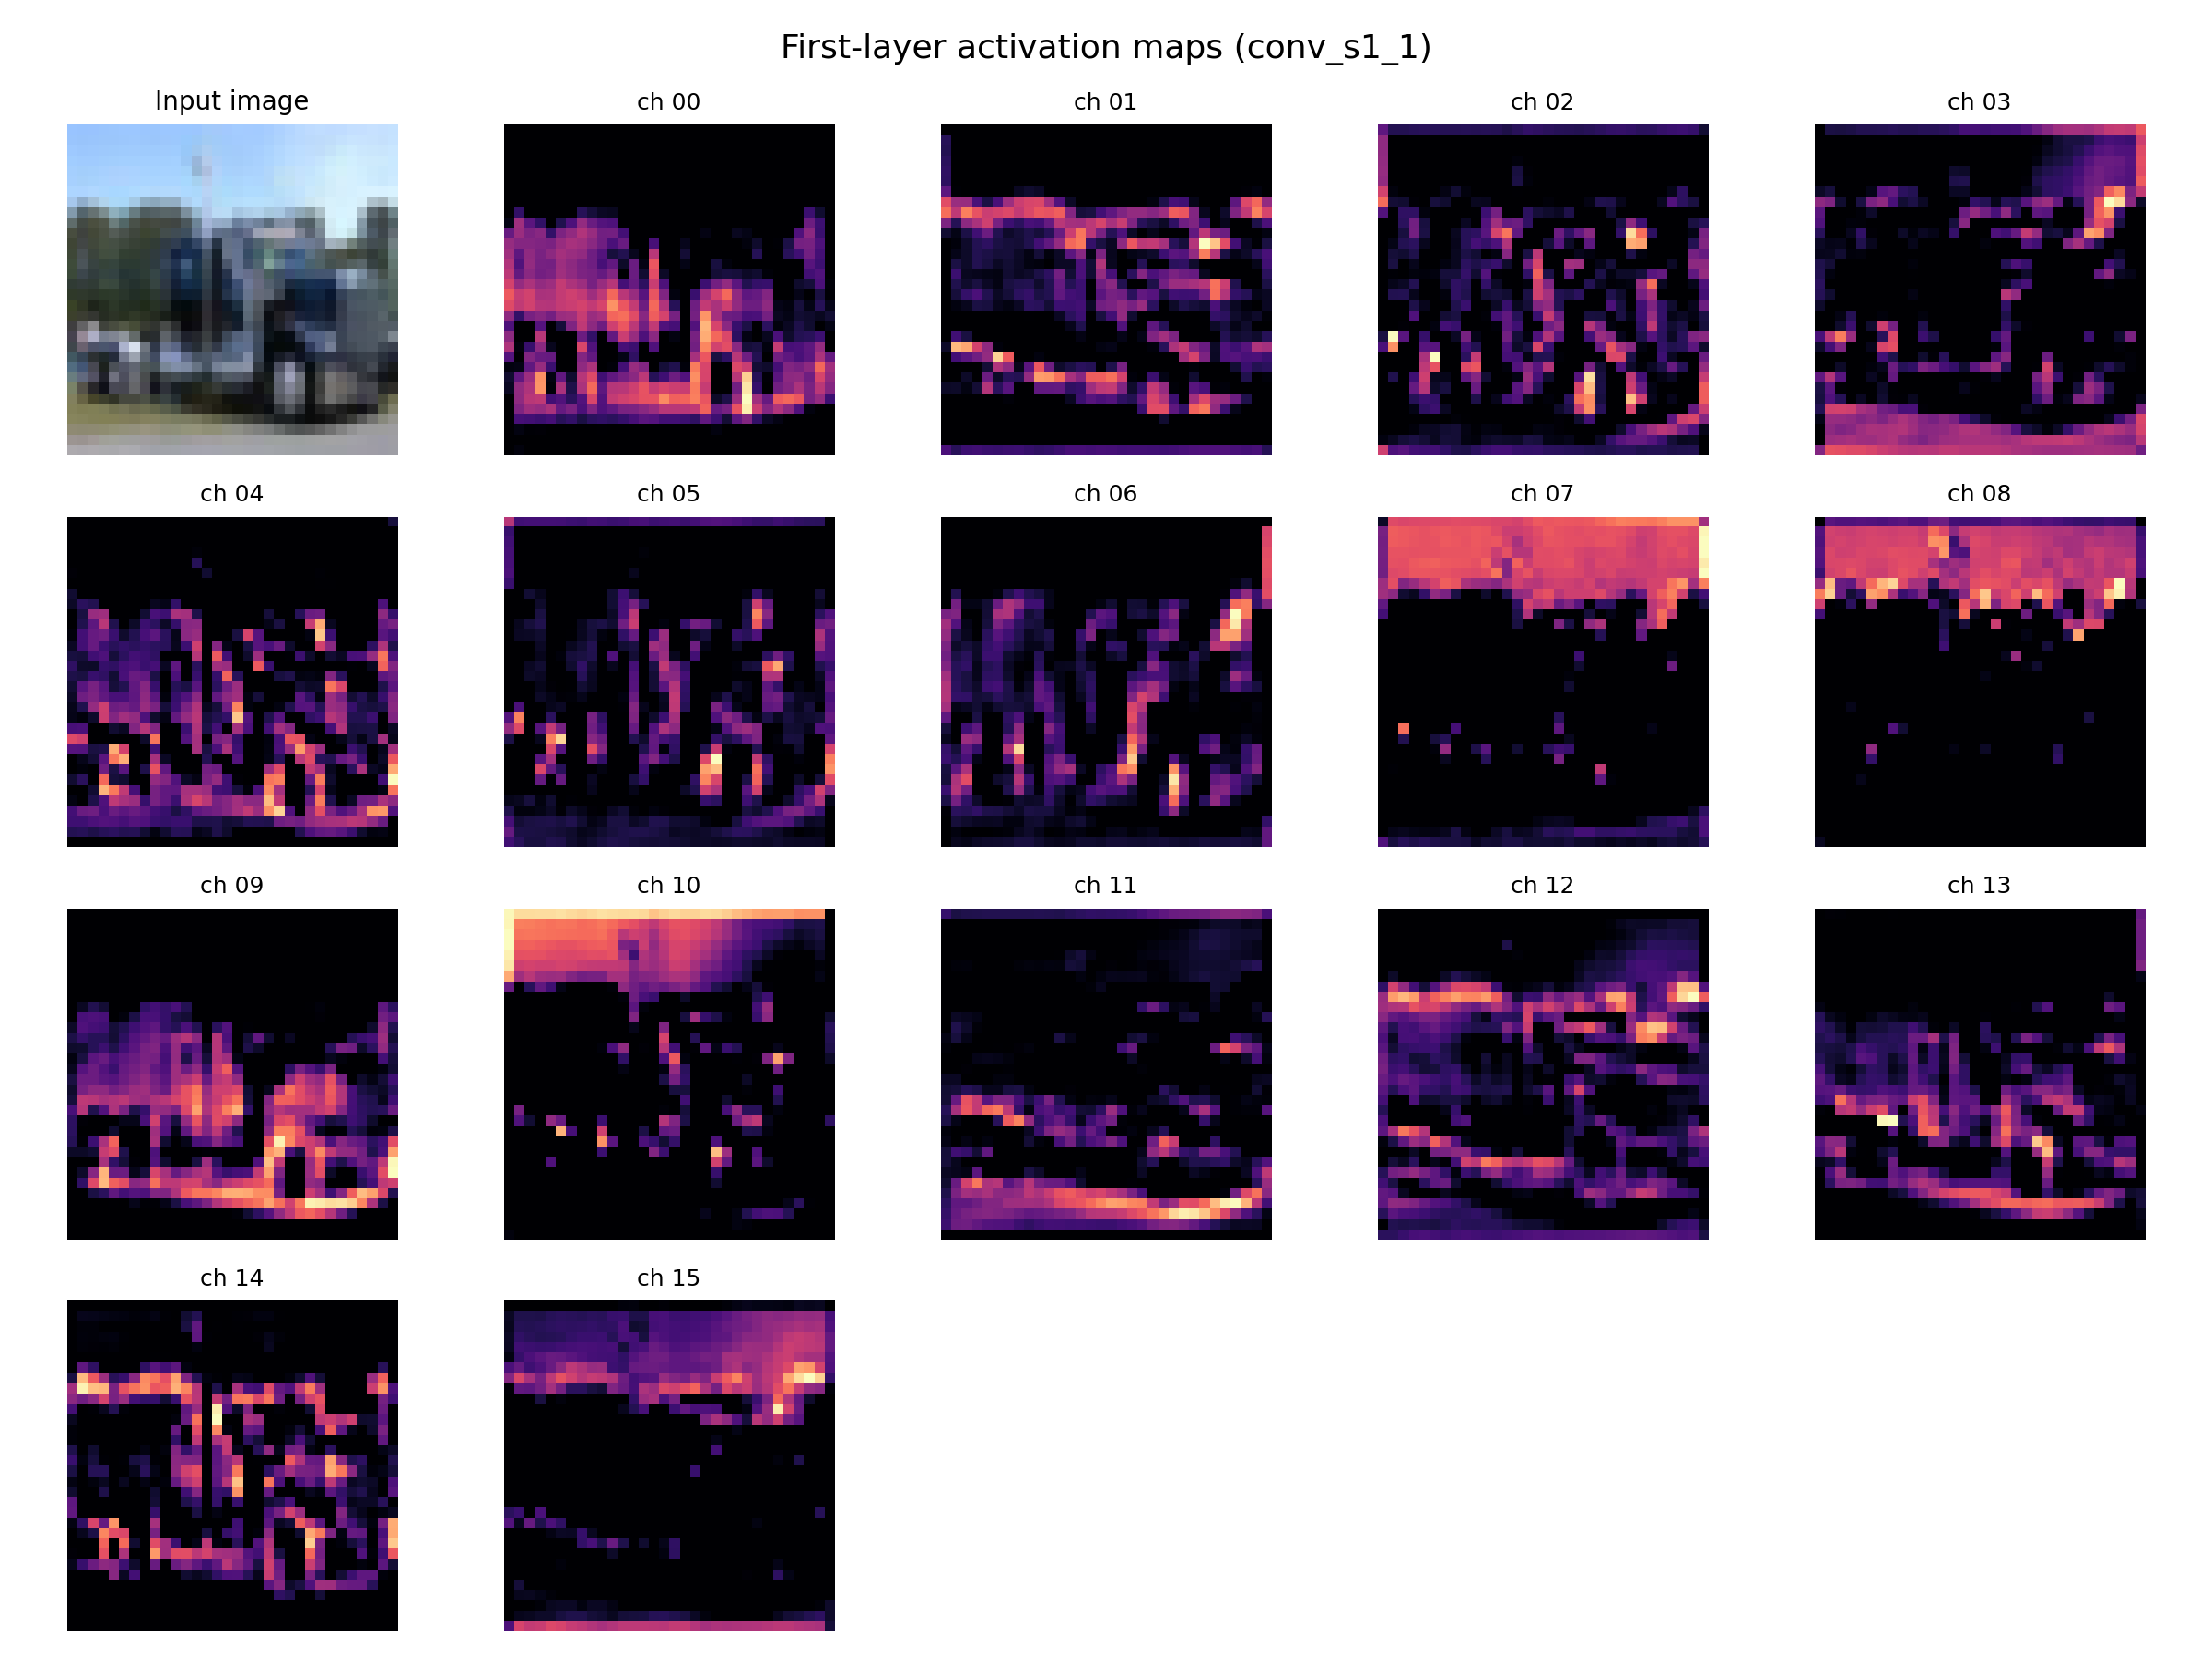
\includegraphics[width=0.5\textwidth]{imgs/section8_first_layer_activation_maps.png}
\caption{Cartes d'activation de la premi\`ere couche \texttt{conv\_s1\_1} pour l'image principale de la classe \textit{truck}. Le texte interne \`a la figure est laiss\'e en anglais pour garantir un rendu stable.}
\label{fig:section8_first_layer}
\end{figure}

\subsection{Cartes d'activation dans les couches profondes du mod\`ele raffin\'e}
L'analyse a ensuite port\'e sur les couches \texttt{conv\_s2\_2} et \texttt{conv\_s3\_2}, qui produisent respectivement des tenseurs de taille $16\times 16\times 32$ et $8\times 8\times 64$. La r\'eduction progressive de r\'esolution due aux op\'erations de \textit{pooling}, d\'ej\`a discut\'ee \`a la Section~6, augmente le champ r\'ecepteur effectif et conduit \`a des repr\'esentations moins directement lisibles \`a l'\'echelle du pixel. La figure~\ref{fig:section8_deep_layers} affiche, pour chaque couche, les $8$ canaux de plus forte activation moyenne sur la m\^eme image.

Par rapport \`a la premi\`ere couche, ces cartes apparaissent plus s\'electives et plus parcimonieuses. Le taux moyen d'activations positives passe de $0.422$ dans \texttt{conv\_s2\_2} \`a $0.402$ dans \texttt{conv\_s3\_2}, et l'entropie spatiale moyenne diminue de $0.780$ \`a $0.679$. Cette \'evolution est coh\'erente avec l'id\'ee d'une extraction hi\'erarchique : certaines cartes interm\'ediaires restent sensibles \`a des structures g\'eom\'etriques larges, alors que plusieurs cartes profondes se concentrent davantage sur des zones compatibles avec la silhouette du camion, ses roues ou l'opposition entre l'objet et l'arri\`ere-plan. Une interpr\'etation s\'emantique directe de chaque canal resterait toutefois excessive, car ces cartes repr\'esentent avant tout des r\'eponses internes utiles \`a la d\'ecision de classification.

\begin{figure}[htbp]
\centering
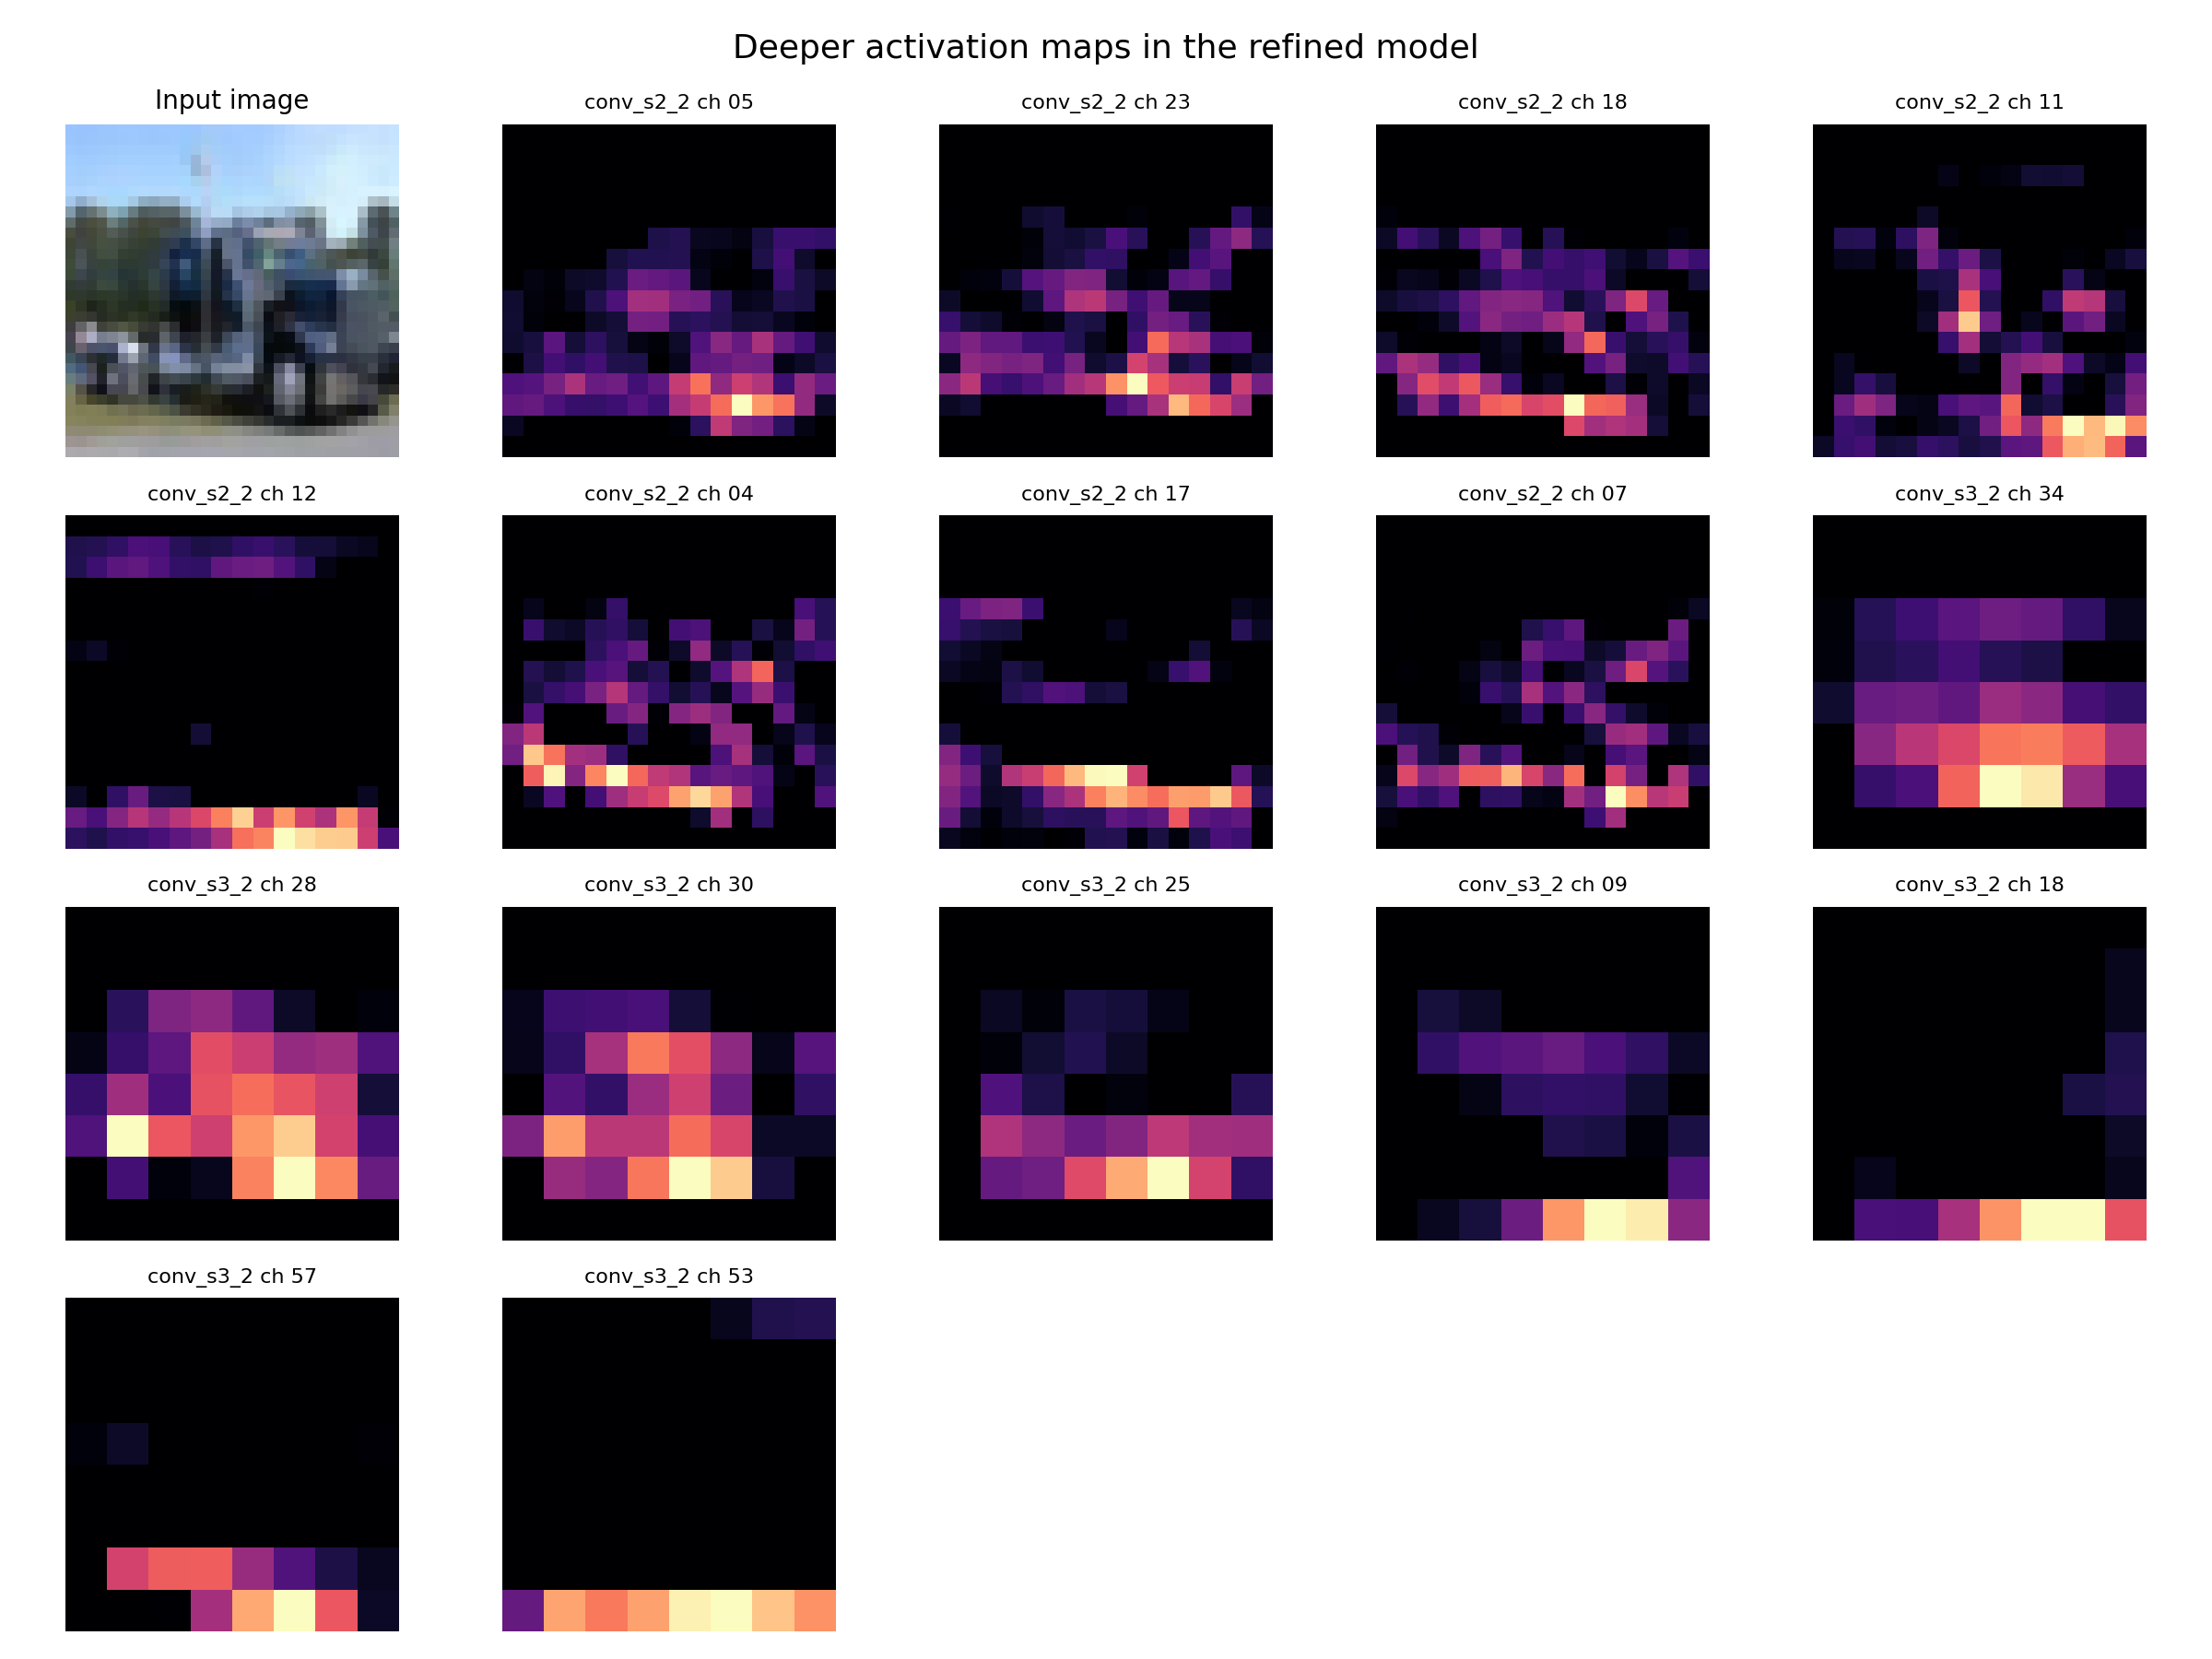
\includegraphics[width=0.5\textwidth]{imgs/section8_deep_layer_activation_maps.png}
\caption{Cartes d'activation de couches profondes du mod\`ele raffin\'e : top-$8$ de \texttt{conv\_s2\_2} et top-$8$ de \texttt{conv\_s3\_2}, class\'es par activation moyenne sur l'image principale.}
\label{fig:section8_deep_layers}
\end{figure}

\subsection{\'Evolution des cartes d'activation pendant l'apprentissage}
Aucun checkpoint exploitable n'\'etait disponible pour le mod\`ele profond final avant cette section ; un run de r\'ef\'erence a donc \'et\'e relanc\'e en sauvegardant uniquement les poids aux epochs $0$, $1$, $5$ et $15$. La comparaison a \'et\'e conduite sur la m\^eme image principale, avec les m\^emes canaux suivis \`a toutes les \'etapes : les canaux $12$ et $6$ de \texttt{conv\_s1\_1}, puis les canaux $34$ et $28$ de \texttt{conv\_s3\_2}, choisis \`a partir du mod\`ele final.

La figure~\ref{fig:section8_evolution} montre qu'\`a l'epoch $0$, avant toute mise \`a jour, les r\'eponses restent diffuses et peu structur\'ees. D\`es l'epoch $1$, certains contrastes spatiaux deviennent visibles, mais les cartes profondes conservent encore une organisation instable. \`A l'epoch $5$, les structures principales se stabilisent, et \`a l'epoch $15$ les cartes profondes apparaissent nettement plus localis\'ees sur des r\'egions discriminantes. Cette structuration progressive se retrouve dans des statistiques simples : l'\'ecart-type moyen des activations suivies n'augmente que de $0.031$ dans \texttt{conv\_s1\_1} entre les epochs $0$ et $15$, contre $0.303$ dans \texttt{conv\_s3\_2}. L'\'evolution des couches profondes est donc plus marqu\'ee que celle de la premi\`ere couche, ce qui sugg\`ere une sp\'ecialisation croissante des repr\'esentations internes au cours de l'apprentissage.

\begin{figure}[htbp]
\centering
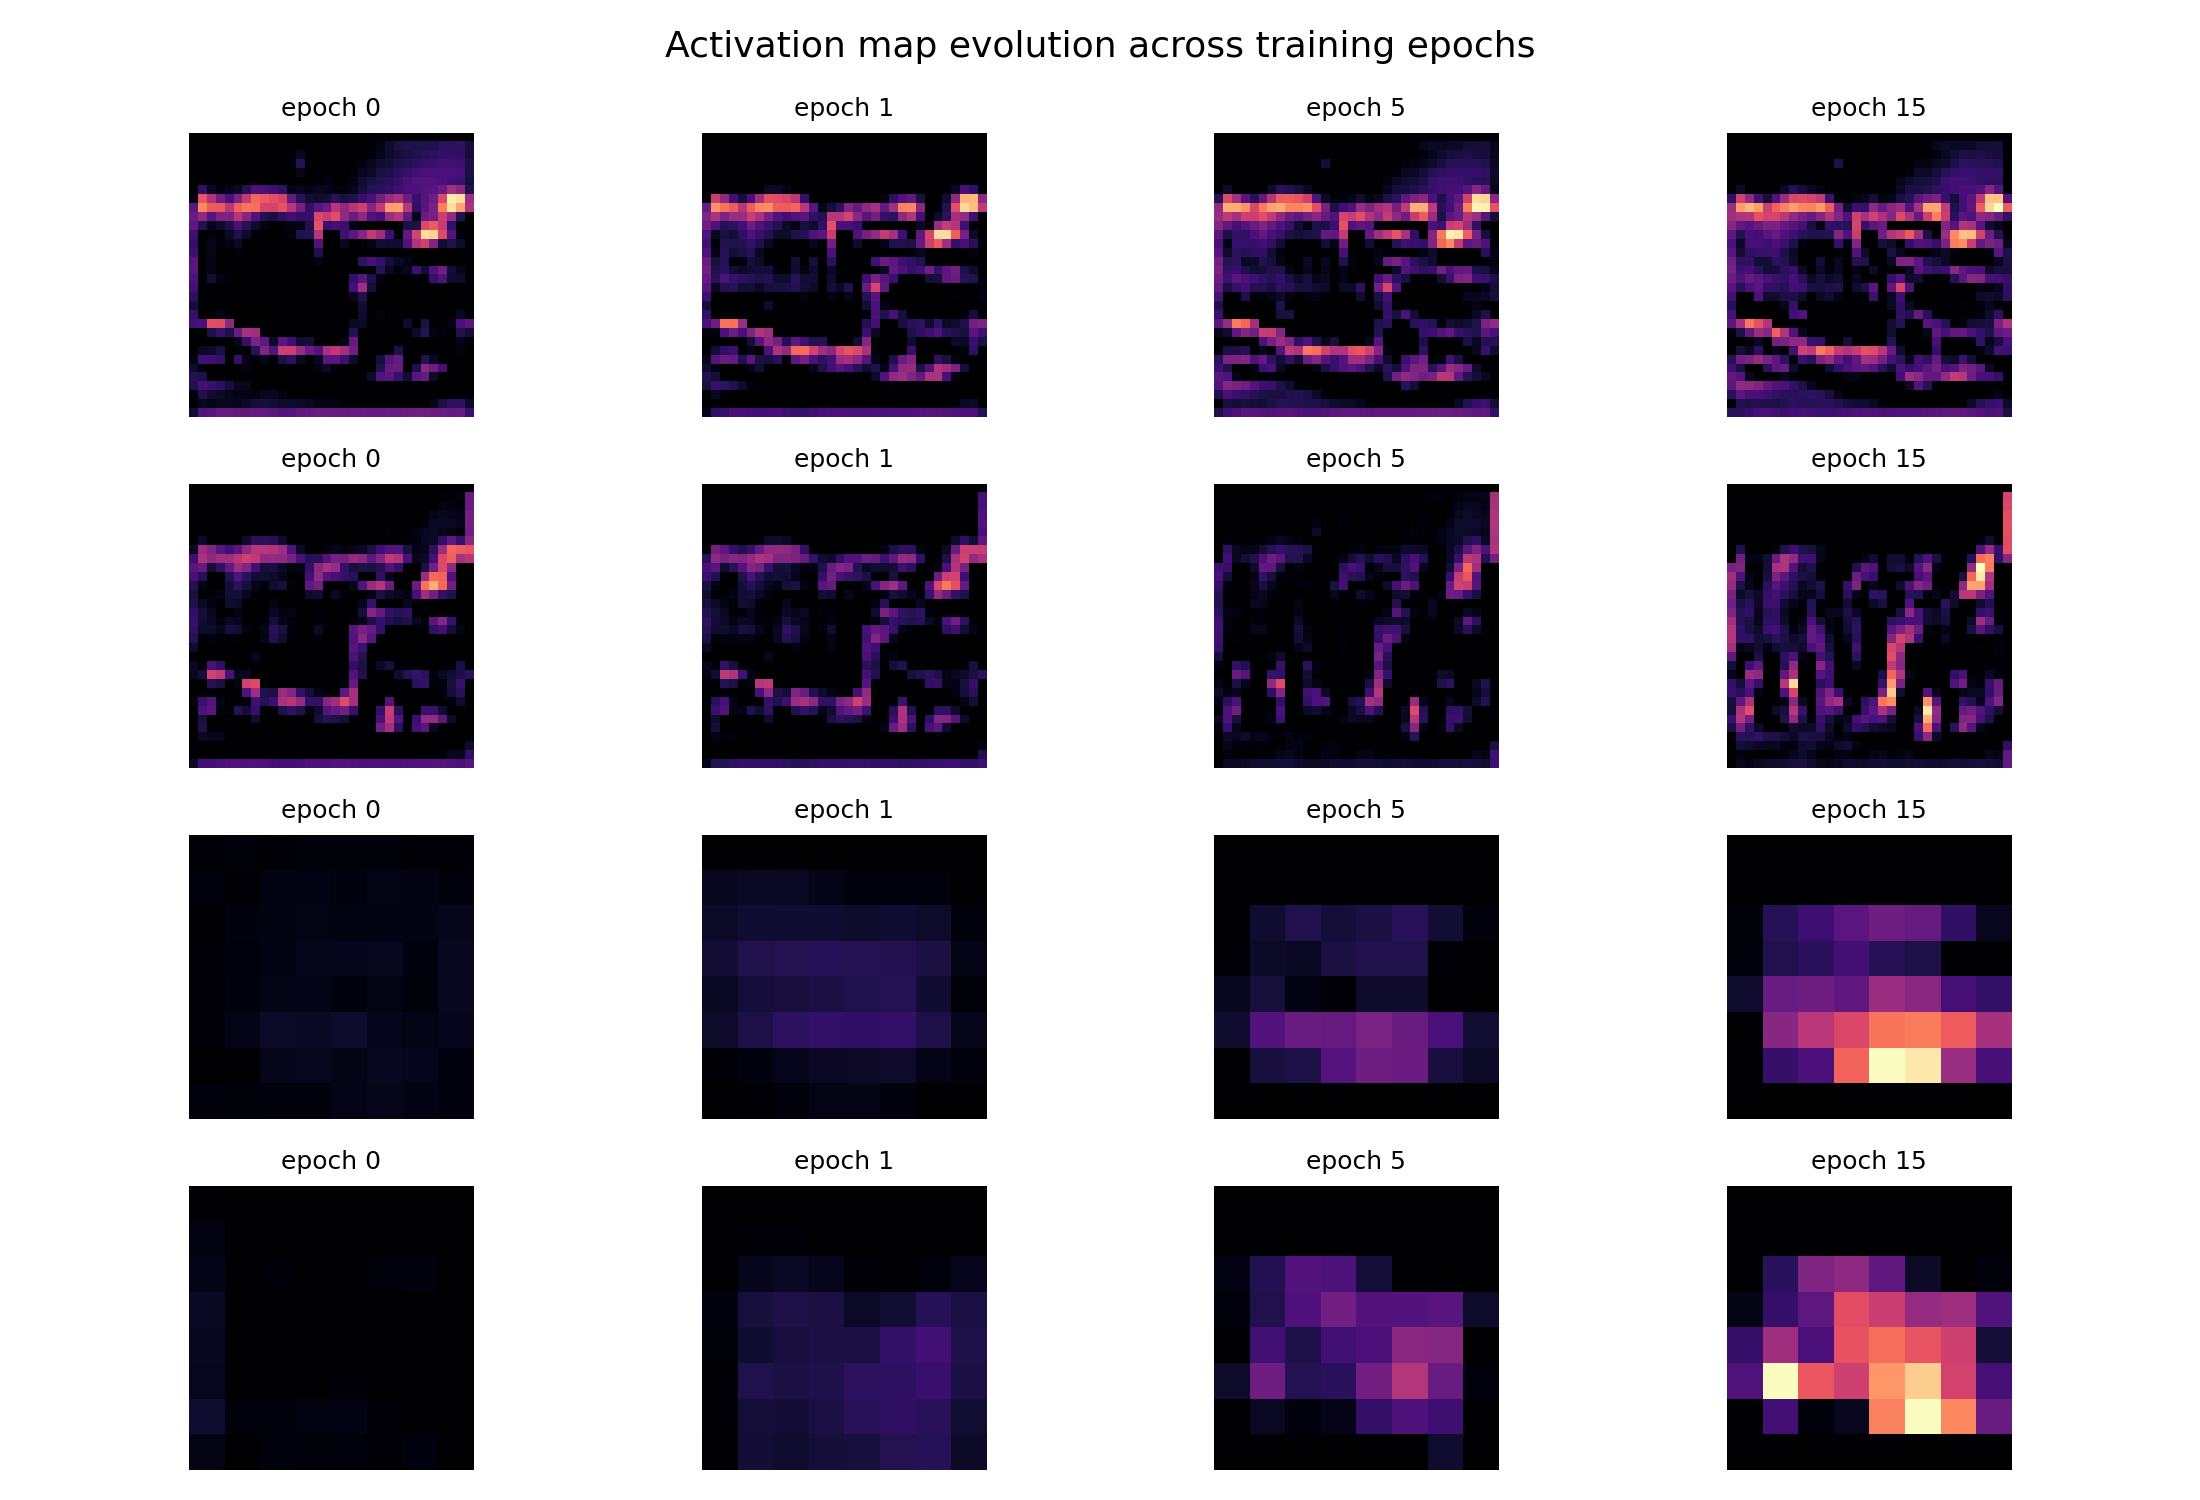
\includegraphics[width=0.5\textwidth]{imgs/section8_activation_evolution.png}
\caption{\'Evolution des cartes d'activation pour des canaux fix\'es de \texttt{conv\_s1\_1} et \texttt{conv\_s3\_2} aux epochs $0$, $1$, $5$ et $15$. La normalisation est fix\'ee par canal sur l'ensemble des epochs afin de rendre la comparaison temporelle lisible.}
\label{fig:section8_evolution}
\end{figure}

\begin{table*}[htbp]
\centering
\caption{Synth\`ese des visualisations retenues pour l'analyse des cartes d'activation.}
\label{tab:section8_summary}
\footnotesize
\begin{tabular}{|p{2.2cm}|p{2.7cm}|p{2.2cm}|p{1.4cm}|p{6.7cm}|}
\hline
Analyse & Couches inspect\'ees & Image retenue & Epochs & Observation concise \\
\hline
Premi\`ere couche & \texttt{conv\_s1\_1} & \textit{truck}, idx. $626$ & $15$ & $16$ cartes encore denses et localement interpr\'etables ; plusieurs canaux soulignent bords et contrastes chromatiques. \\
\hline
Couches profondes & \texttt{conv\_s2\_2}, \texttt{conv\_s3\_2} & \textit{truck}, idx. $626$ & $15$ & Top-$8$ par couche ; activations plus s\'electives et moins entropiques dans \texttt{conv\_s3\_2} que dans \texttt{conv\_s2\_2}. \\
\hline
\'Evolution temporelle & \texttt{conv\_s1\_1}, \texttt{conv\_s3\_2} & \textit{truck}, idx. $626$ & $0,1,5,15$ & M\^emes canaux suivis \`a toutes les \'etapes ; r\'eponses de plus en plus structur\'ees, surtout dans la couche profonde. \\
\hline
\end{tabular}
\end{table*}

\subsection{Discussion et limites d'interpr\'etation}
L'ensemble des visualisations reste coh\'erent avec les choix architecturaux des Sections~6 et~7. Les cartes de la premi\`ere couche traduisent des r\'eponses locales compatibles avec un banc de filtres sensibles aux bords, au contraste et \`a certaines oppositions chromatiques, tandis que les couches profondes deviennent plus s\'electives \`a mesure que le champ r\'ecepteur effectif s'accro\^it. L'\'evolution au cours des epochs montre en outre que les repr\'esentations profondes se structurent beaucoup plus fortement que les r\'eponses de bas niveau, ce qui est compatible avec l'apprentissage progressif de motifs utiles \`a la classification.

Ces cartes ne doivent toutefois pas \^etre sur-interpr\'et\'ees. Les figures reposent sur une normalisation min-max par carte pour les panneaux statiques, puis par canal sur l'ensemble des epochs pour la comparaison temporelle ; elles permettent donc une lecture qualitative, mais pas une comparaison absolue d'amplitude entre tous les canaux. Par ailleurs, une carte d'activation ne fournit pas \`a elle seule une causalit\'e directe sur la d\'ecision finale : elle renseigne sur des r\'eponses internes du r\'eseau, dont une partie seulement peut recevoir une interpr\'etation visuelle explicite. Enfin, le rapport se concentre volontairement sur une image principale pour conserver des figures lisibles ; l'inspection compl\'ementaire d'un exemple correctement class\'e de la classe \textit{frog} dans le notebook confirme les tendances g\'en\'erales, sans supprimer la part d'ambigu\"\i t\'e inh\'erente \`a ce type de visualisation.

\begin{thebibliography}{00}
    
\bibitem{keras_input_layer}
Keras, ``Input object,'' Keras 3 API documentation, accessed Mar. 8, 2026. [Online]. Available: \url{https://keras.io/api/layers/core_layers/input/}

\bibitem{lecun_convolutional_networks}
Y. LeCun, K. Kavukcuoglu, and C. Farabet, ``Convolutional Networks and Applications in Vision,'' presented at ISCAS 2010, accessed Mar. 8, 2026. [Online]. Available: \url{https://cseweb.ucsd.edu/~gary/cs200/s12/lecun-iscas-10.pdf}

\bibitem{cifar10_dataset}
A. Krizhevsky, ``CIFAR-10 and CIFAR-100 datasets,'' accessed Mar. 8, 2026. [Online]. Available: \url{https://www.cs.toronto.edu/~kriz/cifar.html}

\bibitem{keras_conv2d}
Keras, ``Conv2D layer,'' Keras 3 API documentation, accessed Mar. 8, 2026. [Online]. Available: \url{https://keras.io/api/layers/convolution_layers/convolution2d/}

\bibitem{keras_model_training_apis}
Keras, ``Model training APIs,'' Keras 3 API documentation, accessed Mar. 8, 2026. [Online]. Available: \url{https://keras.io/api/models/model_training_apis/}

\bibitem{keras_input_object}
Keras, ``Input object,'' Keras 3 API documentation, accessed Mar. 8, 2026. [Online]. Available: \url{https://keras.io/api/layers/core_layers/input/}
\bibitem{manzanera_classification_apprentissage}
A. Manzanera, ``Classification et apprentissage,'' support de cours, ENSTA Paris, 2026.

\bibitem{poly_chap4_classifml}
A. Manzanera, ``Chapitre 4 -- Classification et apprentissage,'' polycopi\'e de cours, ENSTA Paris, 2026.
\end{thebibliography}
\end{document}

